\documentclass[cn, 11pt, fancy, hide]{elegantbook}

\usepackage{natbib}
\bibliographystyle{apalike}

\hypersetup{
  pdfcreator={LaTeX via pandoc}}


\usepackage{longtable,booktabs}



\setlength{\emergencystretch}{3em}  % prevent overfull lines
\providecommand{\tightlist}{%
  \setlength{\itemsep}{0pt}\setlength{\parskip}{0pt}}

\setcounter{secnumdepth}{5}

%%% Use protect on footnotes to avoid problems with footnotes in titles
\let\rmarkdownfootnote\footnote%
\def\footnote{\protect\rmarkdownfootnote}

  \title{2019年青羊区小学生课业负担分析报告}

\subtitle{四、五年级}

  \author{王敏杰}

  \date{2019-08-22}

% logo 图案
  \logo{figure/logo.png}
% 封面图片
  \cover{figure/cover.jpg}
% 版本号
  \version{3.08}
% 机构名
  \institute{Elegant LaTeX Program}
% 引用格言
  \extrainfo{Victory won't come to us unless we go to it. --- M. Moore}
% 导言区 preamble
\usepackage{framed,color}
\definecolor{shadecolor}{RGB}{248,248,248}

\usepackage{booktabs}
\usepackage{longtable}


\usepackage{array}
\usepackage{multirow}
\usepackage{wrapfig}
\usepackage{float}
\usepackage{colortbl}
\usepackage{pdflscape}
\usepackage{tabu}
\usepackage{threeparttable}
\usepackage{threeparttablex}
\usepackage[normalem]{ulem}
\usepackage{makecell}
\usepackage{xcolor}


\frontmatter

\begin{document}
% 封面
\maketitle
% 插入 before_body.tex

% 目录
{
\setcounter{tocdepth}{2}
\tableofcontents
}
% 表目录
% 图目录
% 书籍主体部分
\mainmatter

\hypersetup{pageanchor=true}

\hypertarget{intro}{%
\chapter{导言}\label{intro}}

2018年12月教育部等九部门印发中小学生减负措施的通知,要求切实减轻违背教育教学规律、有损中小学生身心健康的过重学业负担,促进中小学生健康成长,培养德智体美劳全面发展的社会主义建设者和接班人。我区坚持学生课业负担年度调查,了解相关减负政策的落实情况。2019年6月,对全区四、五、七年级的学生进行了学生课业负担状况问卷调查,分别收到有效数据7912、8018、5146份。本次学生课业负担状况主要考查学生的课业负担状况(包括客观课业负担和主观学习感受)和相关影响因素。通过主客观负担和影响因素数据的呈现,以及分析课业负担、学习方法、学习成绩三者的关联,进一步分析落实减轻学生学业负担、提高学生学习深度的有效路径。

本次学生学业负担评价指标如下表\ref{tab:zb}所示:

\begin{table}[!h]

\caption{\label{tab:zb}学生课业负担评价指标}
\centering
\begin{tabu} to \linewidth {>{\raggedright}X>{\raggedright}X>{\raggedright\arraybackslash}p{10cm}}
\toprule
评价内容 & 关键指标 & 指标解释\\
\midrule
课业负担状况 & 客观学习负担 & 教师拖堂、体育艺术课等学科开齐开足、每天体育锻炼时间、睡眠时间、是否公布成绩及排名、完成家庭作业时间、违规补课的达标情况以及课外补习、课外艺体学习情况。\\
\cmidrule{1-3}
学业负担状况 & 主观学习感受 & 学习活动中所承受的负担感受\\
\cmidrule{1-3}
 & 学习方法 & 作业完成情况、学习深度\\
\cmidrule{2-3}
\multirow[t]{-2}{*}{\raggedright\arraybackslash 影响因素} & 家庭教育 & 父母支持\\
\bottomrule
\end{tabu}
\end{table}

国家、四川省在减轻学生过重课业负担,保障学生身心健康方面有一系列政策要求和规定,依据国家及地方相关政策文件,设置了11道题目通过问卷调查的方式,了解学生的客观学习负担状况。对客观学习负担的题目进行了各选项的频次分析,以调查其符合有关政策规定的情况,即达标情况。具体政策依据和标准如表\ref{tab:zcyj}所示:

\begin{table}[!h]

\caption{\label{tab:zcyj}学生客观学习负担评价政策依据}
\centering
\begin{tabular}{r>{\raggedright\arraybackslash}p{2cm}>{\raggedright\arraybackslash}p{5cm}>{\raggedright\arraybackslash}p{6cm}}
\toprule
序号 & 调查内容 & 评价标准 & 依据\\
\midrule
\rowcolor{gray!6}  1 & 体育课设置 & 小学3-6年级和初中每周3课时 & 《中共中央国务院关于加强青少年体育增强青少年体质的意见》\\
2 & 音乐课设置 & 严格执行国家课程方案和课程标准,开足开齐规定课程,努力提高教学质量,促进学生全面发展。 & 《中小学生减负措施》(减负三十条)\\
\rowcolor{gray!6}  3 & 美术课设置 & 严格执行国家课程方案和课程标准,开足开齐规定课程,努力提高教学质量,促进学生全面发展。 & 《中小学生减负措施》(减负三十条)\\
4 & 信息技术课设置 & 严格执行国家课程方案和课程标准,开足开齐规定课程,努力提高教学质量,促进学生全面发展。 & 《中小学生减负措施》(减负三十条)\\
\rowcolor{gray!6}  5 & 劳动与技术课设置 & 严格执行国家课程方案和课程标准,开足开齐规定课程,努力提高教学质量,促进学生全面发展。 & 《中小学生减负措施》(减负三十条)\\
\addlinespace
6 & 体育锻炼时间 & 确保每天锻炼1小时,条件允许的情况下尽量安排在户外。 & 《中小学生减负措施》(减负三十条)\\
\rowcolor{gray!6}  7 & 学生睡眠时间 & 保证小学生每天睡眠时间不少于10个小时,初中生不少于9个小时, & 《中小学生减负措施》(减负三十条)\\
8 & 学生作业负担 & 小学一二年级不布置书面家庭作业,三至六年级家庭作业不超过60分钟,初中家庭作业不超过90分钟, & 《中小学生减负措施》(减负三十条)\\
\rowcolor{gray!6}  9 & 成绩公布排名 & 考试成绩实行等级评价,严禁以任何形式、方式公布学生考试成绩及排名。 & 《中小学生减负措施》(减负三十条)\\
10 & 拖堂情况 & 改进教学方法,提高课堂教学的质量和效率,切实做到不拖堂 & 《中小学学生近视眼防控工作方案》\\
\addlinespace
\rowcolor{gray!6}  11 & 违规补课 & 严禁学校以任何名目(包括家长委员会等) 占用双休日、节假日、寒暑假组织学生集体补课或上新课 & 四川省教育厅关于贯彻《四川省人民政府办公厅关于规范办学行为深入推进素质教育的意见》的实施意见\\
\bottomrule
\end{tabular}
\end{table}

\hypertarget{section}{%
\chapter{四年级课业负担状况}\label{section}}

\hypertarget{section-1}{%
\section{主要结论}\label{section-1}}

\begin{enumerate}
\def\labelenumi{\arabic{enumi}.}
\item
  在区域层面, ``违规补课''、``信息技术课程开设开足'' 两个方面的平均达标率均在 80\% 以上,但 ``不公布成绩'' 的达标率不足 30\%,``平均家庭作业不超过 1 小时'' 的达标率低于 50\%。 在学校层面,针对客观学习负担 11 个指标,全区 34 所学校中,金沙小学 、实验小学 、同辉(国际)学校 3所学校所有指标的达标率都高于全区平均达标率;东城根街小学、鼓楼小学、泡桐树小学、实小青华分校 、实验小学成飞分校、实验小学明道分校、万春小学7所学校只有一个或两个指标低于全区平均达标率;新华路小学、文翁实验小学、双眼井小学、实验小学战旗分校、实验小学文苑分校、清波小学校、泡桐树小学境界分校7所学校所有指标的达标率均低于全区平均达标率。
\item
  四年级学生的整体主观学习压力不大,课后学习时间基本在能承受的范围内。
\item
  四年级学生学习深度的得分率为 66.49\%,学生学习的深度仍需提高。约40\%的家长会在家陪伴孩子学习。
\item
  数据整体趋势表明,四年级成绩相对较好的学生主要集中在睡眠时间和体育锻炼时间长、压力感受较低和学习深度得分率较高的区域,客观负担达标率高低都有。
\item
  与去年相比,全区11个客观学习负担指标中9个指标的达标率提高,2个指标降低,学生客
  观学习负担整体上降低。
\end{enumerate}

\hypertarget{section-2}{%
\section{客观学习负担情况}\label{section-2}}

\hypertarget{section-3}{%
\subsection{指标达标率情况}\label{section-3}}

在区域层面,全区四年级在``违规补课''、``信息技术课程开设开足''两个方面达标率均在80\%以上,说明较好地遵循了国家或地方有关政策规定的标准和规范。但``不公布成绩''的达标率不足30\%,``平均家庭作业不超过1小时''的达标率低于50\%,对相关政策规定贯彻落实力度还需要大大增强。

\begin{center}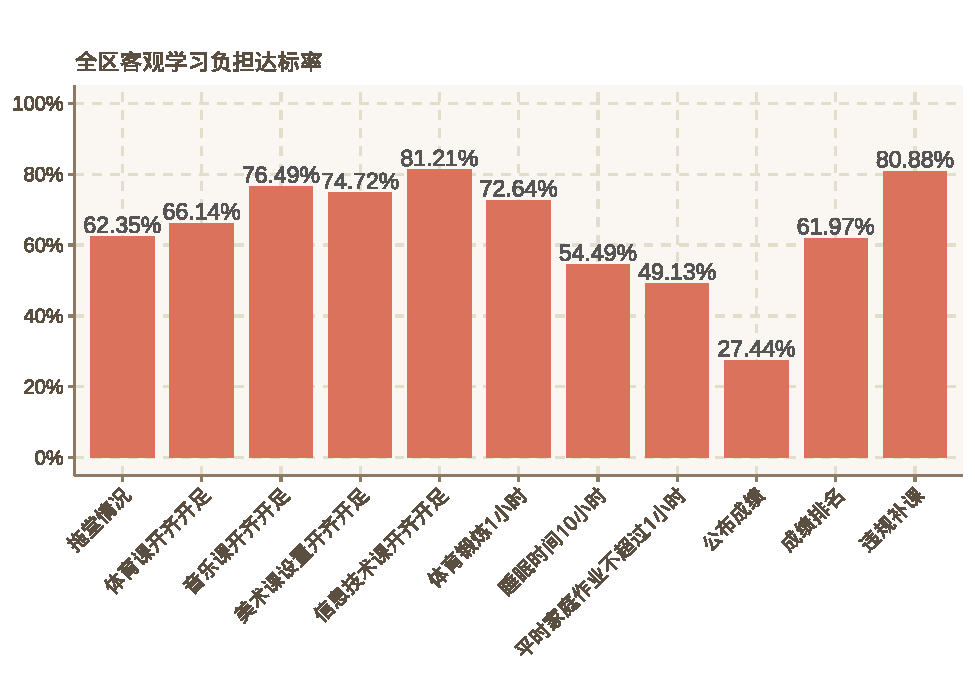
\includegraphics[width=0.99\linewidth]{ElegantBookdown_files/figure-latex/unnamed-chunk-9-1} \end{center}

根据调查结果,语文、数学、英语、其他学科的拖堂比率分别为18.36\%、26.19\%、8.40\%、7.05\%。

\begin{center}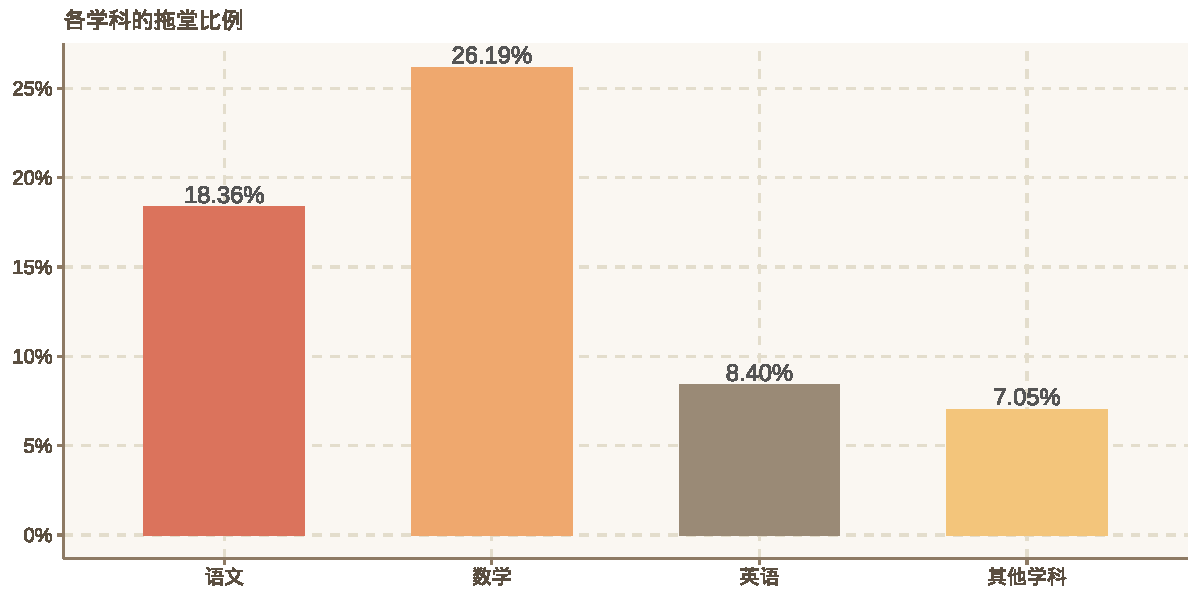
\includegraphics[width=0.99\linewidth]{ElegantBookdown_files/figure-latex/unnamed-chunk-10-1} \end{center}

根据调查结果,仍然存在少量根据考试成绩给学生排座次的情况。

\begin{center}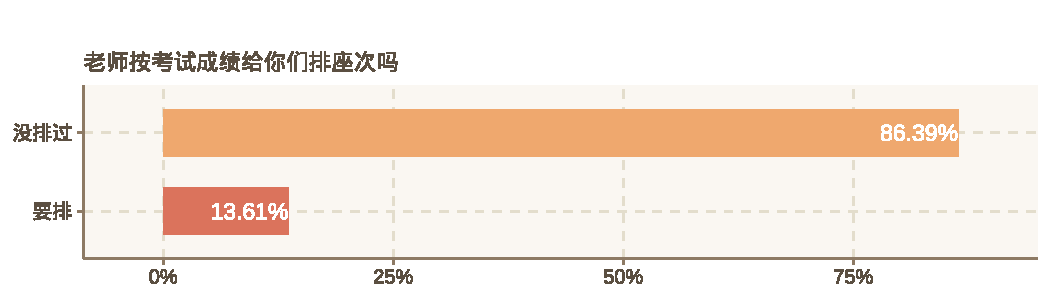
\includegraphics[width=0.99\linewidth]{ElegantBookdown_files/figure-latex/unnamed-chunk-11-1} \end{center}

在学校层面,针对客观学习负担 11 个指标,全区 34 所学校中,金沙小学 、实验小学 、同辉(国际)学校 3所学校所有指标的达标率都高于全区平均达标率;东城根街小学、鼓楼小学、泡桐树小学、实小青华分校 、实验小学成飞分校、实验小学明道分校、万春小学7所学校只有一个或两个指标低于全区平均达标率;新华路小学、文翁实验小学、双眼井小学、实验小学战旗分校、实验小学文苑分校、清波小学校、泡桐树小学境界分校7所学校所有指标的达标率均低于全区平均达标率。

\begin{center}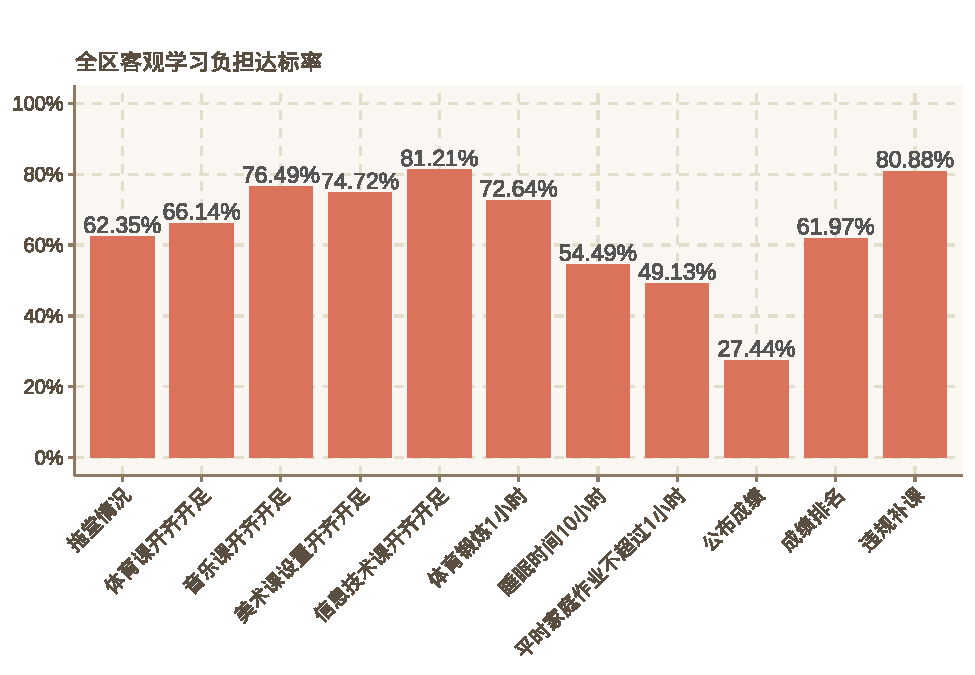
\includegraphics[width=0.99\linewidth]{ElegantBookdown_files/figure-latex/unnamed-chunk-12-1} \end{center}

\hypertarget{section-4}{%
\subsection{课外学习情况}\label{section-4}}

近80\%的四年级学生参加了至少一门文化补课,近70\%的学生一周平均文化补课时间在0-3小时之间,约70\%的学生每天文化补课作业时间在1小时内,参加文化补课的主要原因是扩展知识、拓展能力。

\begin{center}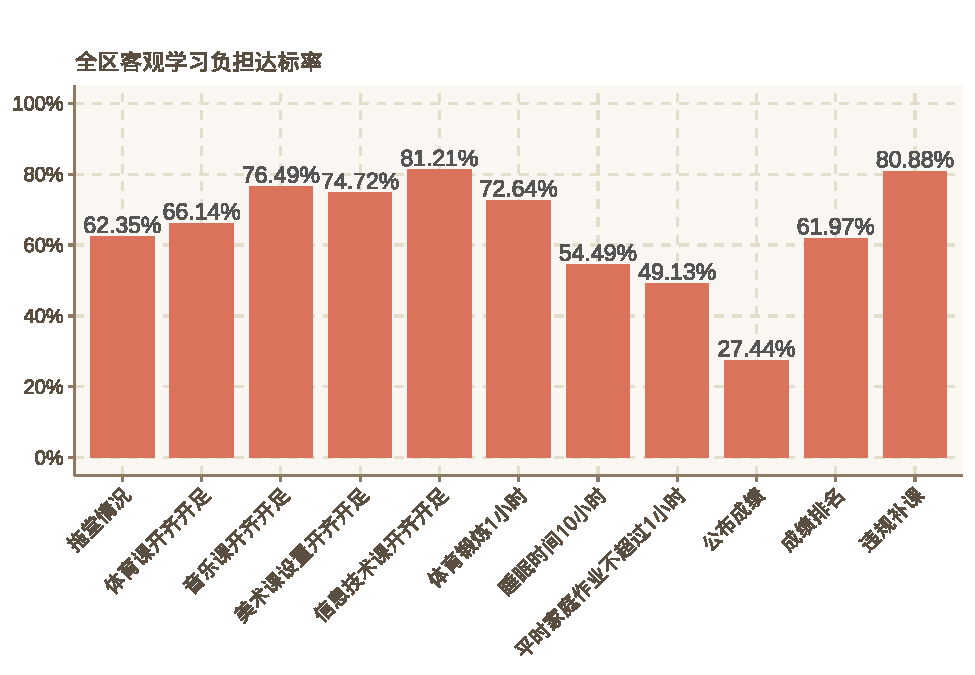
\includegraphics[width=0.99\linewidth]{ElegantBookdown_files/figure-latex/unnamed-chunk-13-1} \end{center}

\begin{center}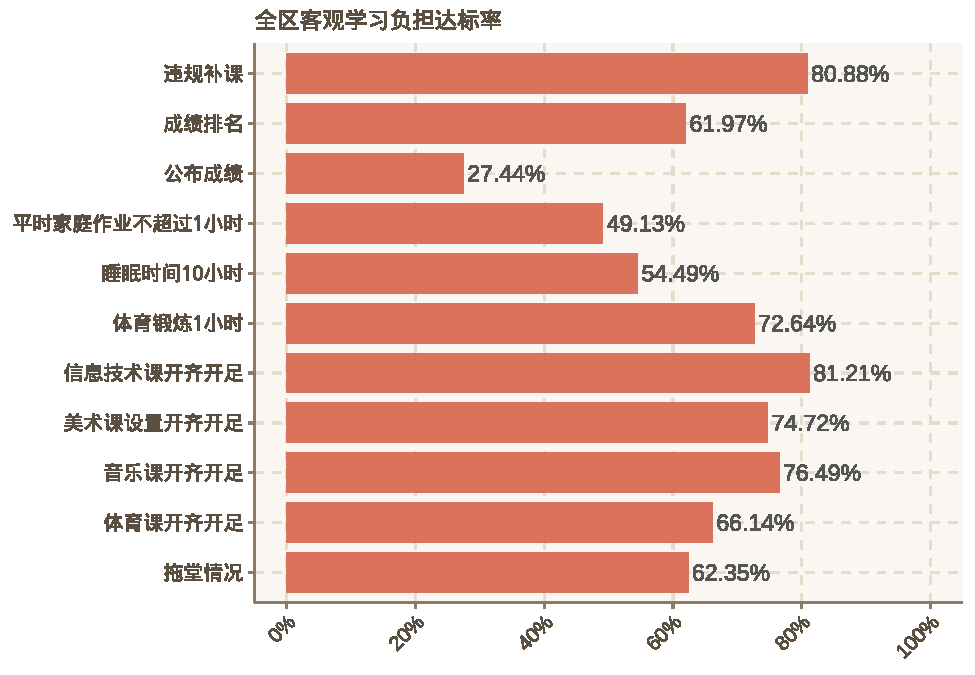
\includegraphics[width=0.99\linewidth]{ElegantBookdown_files/figure-latex/unnamed-chunk-14-1} \end{center}

四年级81.95\% 的学生参加了至少一项艺体培训,近 70\% 的学生一周平均艺体培训时间在 1.5-2 小时之间。

\begin{center}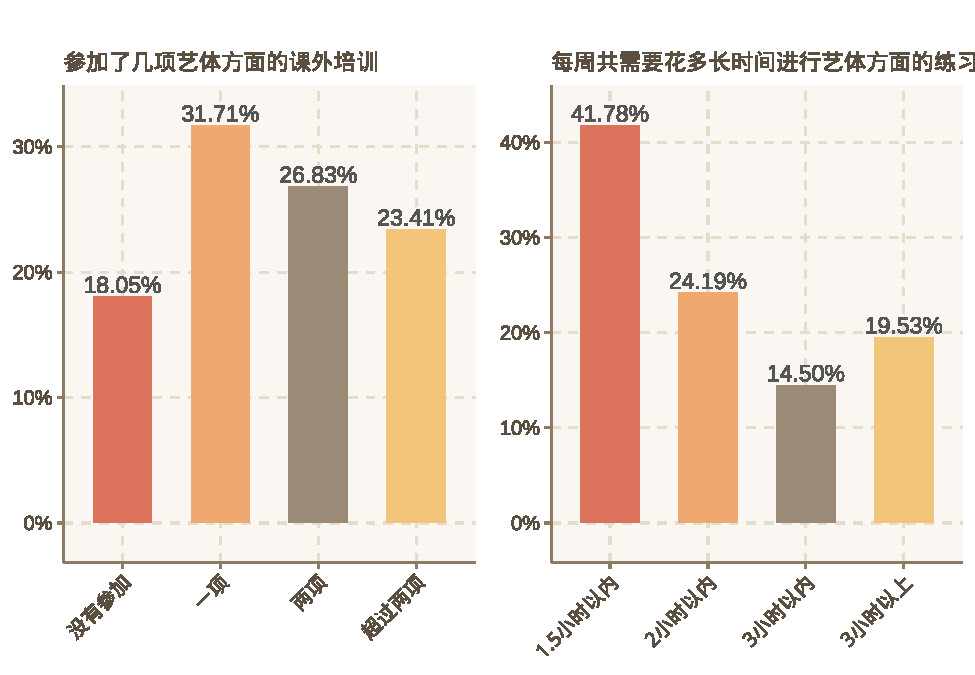
\includegraphics[width=0.99\linewidth]{ElegantBookdown_files/figure-latex/unnamed-chunk-15-1} \end{center}

\hypertarget{section-5}{%
\section{主观学习感受}\label{section-5}}

四年级学生的整体主观学习压力不大,43.16\% 的学生没有压力,47.02\% 的学生有一些压力但仍喜欢学习,22.02\%的学生认为学校和课外学习加在一起才有负担,主要的学习压力来自自己。

\begin{center}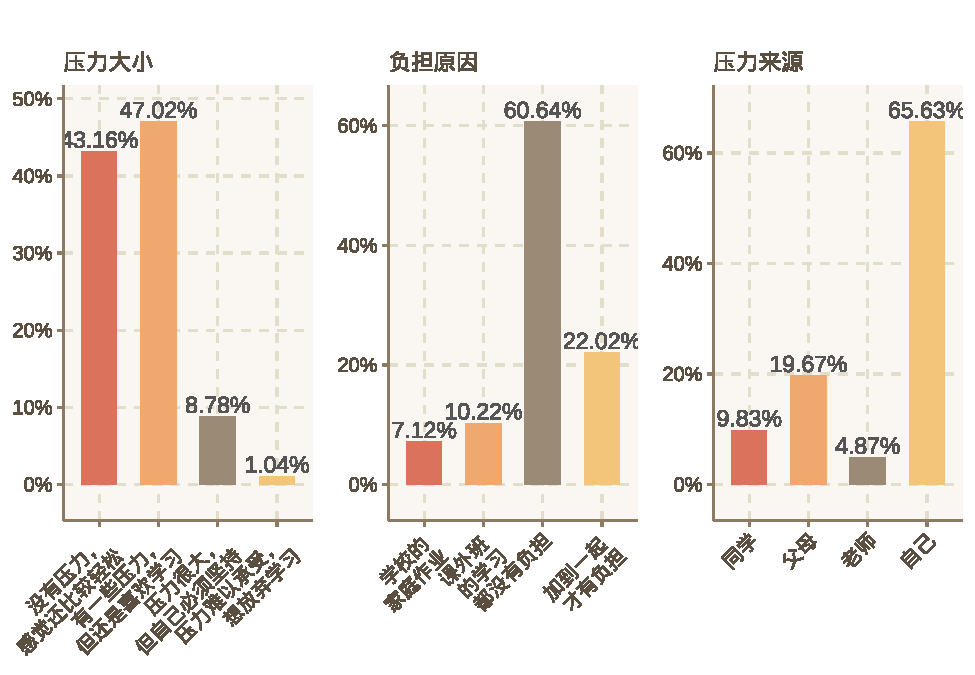
\includegraphics[width=0.99\linewidth]{ElegantBookdown_files/figure-latex/unnamed-chunk-16-1} \end{center}

各校学生学习感知的压力大小分类统计如下:

\begin{center}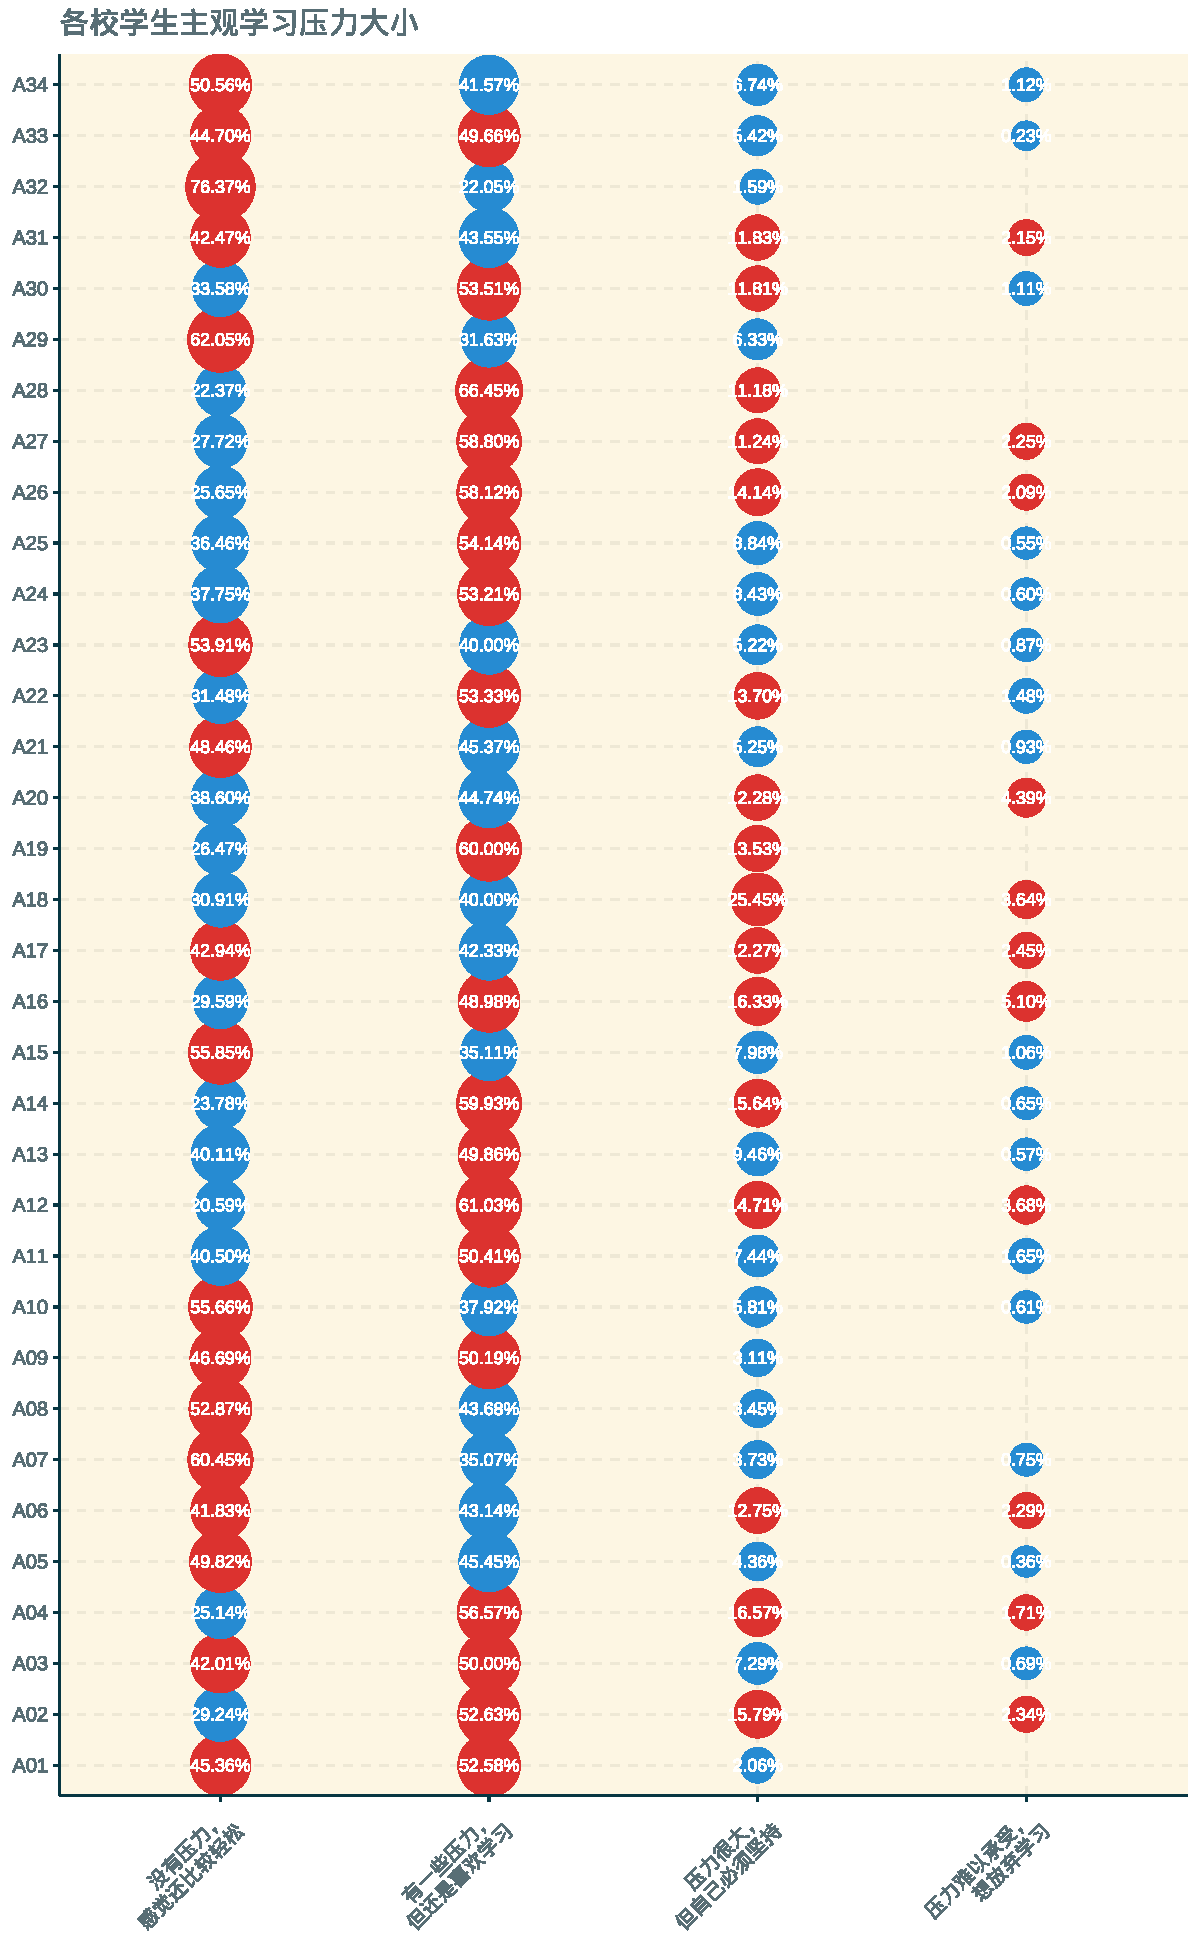
\includegraphics[width=0.99\linewidth]{ElegantBookdown_files/figure-latex/unnamed-chunk-18-1} \end{center}

大部分四年级学生对文化补课和艺体培训接受度和兴趣比较高。

\begin{center}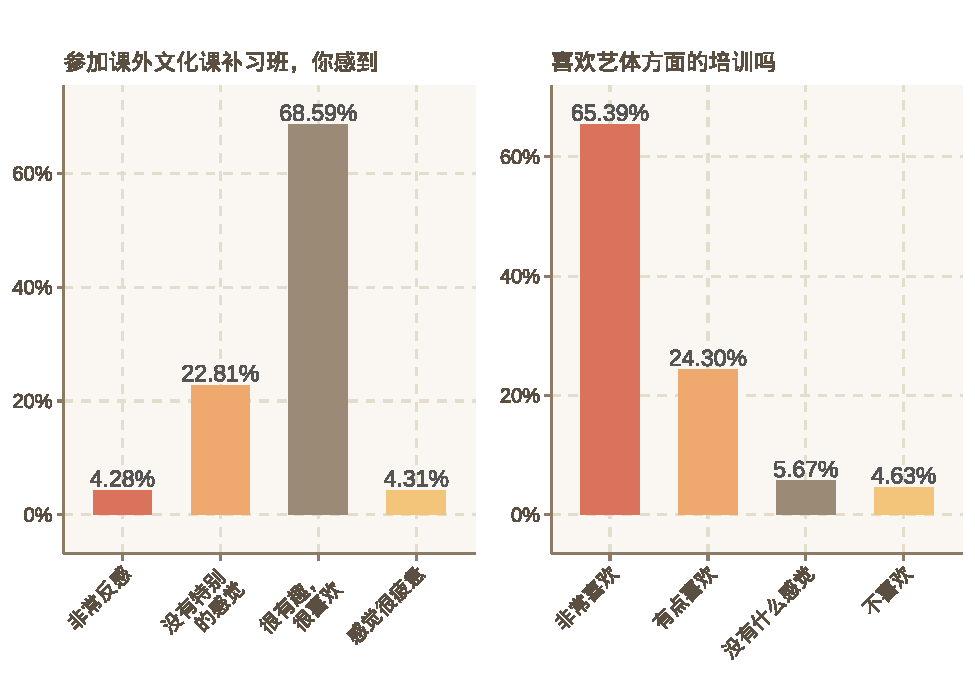
\includegraphics[width=0.99\linewidth]{ElegantBookdown_files/figure-latex/unnamed-chunk-19-1} \end{center}

将完成所有学校作业、补习班课程、补习班作业、艺体方面的练习的时间加和,与学生可以接受的负担时间进行比较,从全区来看,学生心理预期承受时间为平均每周12.63小时,实际支出实际12.06小时,两者相差不大,表明平均而言放学后的学业负荷学生基本能承受。

各校学生实际课后学习时间和能承受的时间及其差值统计如下:

\begin{table}[!h]

\caption{\label{tab:unnamed-chunk-22}各校课外补习实际支出时间与心理预期统计}
\centering
\fontsize{12}{14}\selectfont
\begin{tabular}{lccc}
\toprule
学校 & \makecell[c]{每周实际 \\ 补习时间} & \makecell[c]{每周可承受 \\ 补习时间} & \makecell[c]{超过可承受 \\ 时间}\\
\midrule
\rowcolor{gray!6}  A01 & 10.33 & 11.97 & \multicolumn{1}{r}{\cellcolor[HTML]{F3C57B}{\textcolor{black}{-1.64}}}\\
A02 & 13.83 & 12.40 & \multicolumn{1}{r}{\cellcolor[HTML]{db735c}{\textcolor{black}{1.42}}}\\
\rowcolor{gray!6}  A03 & 11.48 & 12.52 & \multicolumn{1}{r}{\cellcolor[HTML]{F3C57B}{\textcolor{black}{-1.04}}}\\
A04 & 12.85 & 11.33 & \multicolumn{1}{r}{\cellcolor[HTML]{db735c}{\textcolor{black}{1.52}}}\\
\rowcolor{gray!6}  A05 & 10.37 & 11.87 & \multicolumn{1}{r}{\cellcolor[HTML]{F3C57B}{\textcolor{black}{-1.49}}}\\
A06 & 12.40 & 11.40 & \multicolumn{1}{r}{\cellcolor[HTML]{db735c}{\textcolor{black}{1}}}\\
\rowcolor{gray!6}  A07 & 9.80 & 12.30 & \multicolumn{1}{r}{\cellcolor[HTML]{F3C57B}{\textcolor{black}{-2.51}}}\\
A08 & 9.71 & 12.91 & \multicolumn{1}{r}{\cellcolor[HTML]{F3C57B}{\textcolor{black}{-3.2}}}\\
\rowcolor{gray!6}  A09 & 11.46 & 12.43 & \multicolumn{1}{r}{\cellcolor[HTML]{F3C57B}{\textcolor{black}{-0.96}}}\\
A10 & 11.45 & 12.66 & \multicolumn{1}{r}{\cellcolor[HTML]{F3C57B}{\textcolor{black}{-1.21}}}\\
\rowcolor{gray!6}  A11 & 14.09 & 13.04 & \multicolumn{1}{r}{\cellcolor[HTML]{db735c}{\textcolor{black}{1.05}}}\\
A12 & 13.15 & 12.04 & \multicolumn{1}{r}{\cellcolor[HTML]{db735c}{\textcolor{black}{1.11}}}\\
\rowcolor{gray!6}  A13 & 11.71 & 11.62 & \multicolumn{1}{r}{\cellcolor[HTML]{db735c}{\textcolor{black}{0.09}}}\\
A14 & 13.28 & 12.29 & \multicolumn{1}{r}{\cellcolor[HTML]{db735c}{\textcolor{black}{0.99}}}\\
\rowcolor{gray!6}  A15 & 11.99 & 13.46 & \multicolumn{1}{r}{\cellcolor[HTML]{F3C57B}{\textcolor{black}{-1.48}}}\\
A16 & 11.19 & 10.41 & \multicolumn{1}{r}{\cellcolor[HTML]{db735c}{\textcolor{black}{0.78}}}\\
\rowcolor{gray!6}  A17 & 12.30 & 11.47 & \multicolumn{1}{r}{\cellcolor[HTML]{db735c}{\textcolor{black}{0.83}}}\\
A18 & 11.42 & 11.64 & \multicolumn{1}{r}{\cellcolor[HTML]{F3C57B}{\textcolor{black}{-0.21}}}\\
\rowcolor{gray!6}  A19 & 12.76 & 12.56 & \multicolumn{1}{r}{\cellcolor[HTML]{db735c}{\textcolor{black}{0.2}}}\\
A20 & 14.15 & 12.55 & \multicolumn{1}{r}{\cellcolor[HTML]{db735c}{\textcolor{black}{1.59}}}\\
\rowcolor{gray!6}  A21 & 11.08 & 12.77 & \multicolumn{1}{r}{\cellcolor[HTML]{F3C57B}{\textcolor{black}{-1.68}}}\\
A22 & 13.10 & 12.30 & \multicolumn{1}{r}{\cellcolor[HTML]{db735c}{\textcolor{black}{0.81}}}\\
\rowcolor{gray!6}  A23 & 10.25 & 12.15 & \multicolumn{1}{r}{\cellcolor[HTML]{F3C57B}{\textcolor{black}{-1.91}}}\\
A24 & 13.25 & 12.62 & \multicolumn{1}{r}{\cellcolor[HTML]{db735c}{\textcolor{black}{0.63}}}\\
\rowcolor{gray!6}  A25 & 10.87 & 12.37 & \multicolumn{1}{r}{\cellcolor[HTML]{F3C57B}{\textcolor{black}{-1.5}}}\\
A26 & 13.43 & 12.64 & \multicolumn{1}{r}{\cellcolor[HTML]{db735c}{\textcolor{black}{0.79}}}\\
\rowcolor{gray!6}  A27 & 13.72 & 12.54 & \multicolumn{1}{r}{\cellcolor[HTML]{db735c}{\textcolor{black}{1.18}}}\\
A28 & 14.41 & 13.20 & \multicolumn{1}{r}{\cellcolor[HTML]{db735c}{\textcolor{black}{1.21}}}\\
\rowcolor{gray!6}  A29 & 11.79 & 14.48 & \multicolumn{1}{r}{\cellcolor[HTML]{F3C57B}{\textcolor{black}{-2.68}}}\\
A30 & 13.70 & 13.25 & \multicolumn{1}{r}{\cellcolor[HTML]{db735c}{\textcolor{black}{0.46}}}\\
\rowcolor{gray!6}  A31 & 11.00 & 11.53 & \multicolumn{1}{r}{\cellcolor[HTML]{F3C57B}{\textcolor{black}{-0.53}}}\\
A32 & 10.66 & 15.20 & \multicolumn{1}{r}{\cellcolor[HTML]{F3C57B}{\textcolor{black}{-4.54}}}\\
\rowcolor{gray!6}  A33 & 11.48 & 12.44 & \multicolumn{1}{r}{\cellcolor[HTML]{F3C57B}{\textcolor{black}{-0.95}}}\\
A34 & 10.46 & 11.28 & \multicolumn{1}{r}{\cellcolor[HTML]{F3C57B}{\textcolor{black}{-0.82}}}\\
\bottomrule
\multicolumn{4}{l}{\textsuperscript{a} 单位:小时}\\
\end{tabular}
\end{table}

\cleardoublepage

\hypertarget{section-6}{%
\section{学习方法}\label{section-6}}

\hypertarget{section-7}{%
\subsection{学生学习深度}\label{section-7}}

对考查学生学习深度的量表式题目进行因素分析,根据因素分析得到的因子载荷合成学习深度总分,计算得到学生学习深度得分率。全区四年级学生学习深度的得分率为66.49\%,整
体并不高,表明学生学习的深度不够。各校得分率最高的为 77.21\%,最低的为 52.35\%,具体得分率如下:

\begin{center}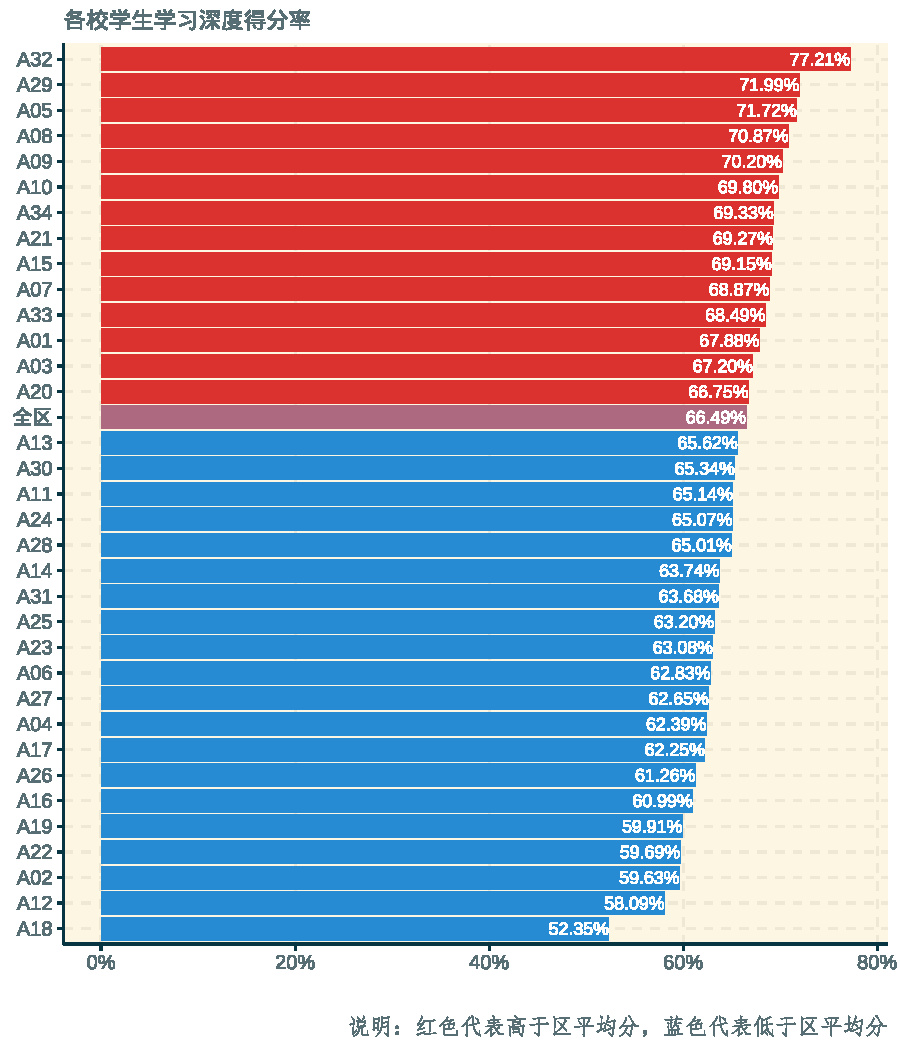
\includegraphics[width=0.99\linewidth]{ElegantBookdown_files/figure-latex/unnamed-chunk-25-1} \end{center}

\hypertarget{section-8}{%
\subsection{学生作业完成情况}\label{section-8}}

对于学生完成作业,超80\%的学生都认为自己是专心致志一鼓作气做完,在正确率方面差别不大。值得注意的是,约60\%学生认为考试比课堂内容和家庭作业灵活一些。此外,41.05\%的家长会在家陪伴孩子学习。

\begin{center}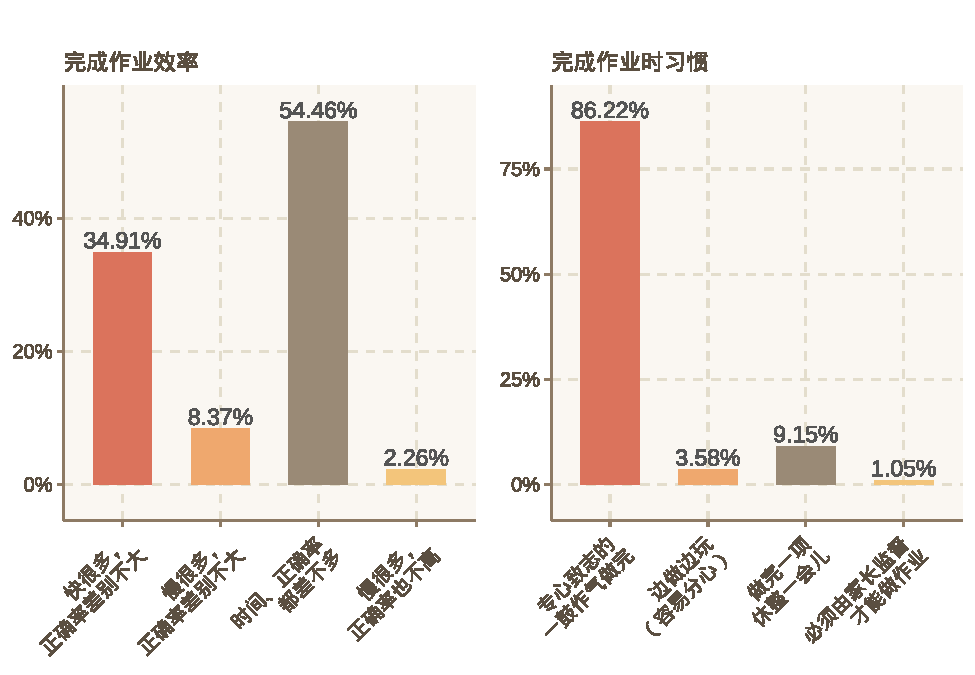
\includegraphics[width=0.99\linewidth]{ElegantBookdown_files/figure-latex/unnamed-chunk-26-1} \end{center}

\begin{center}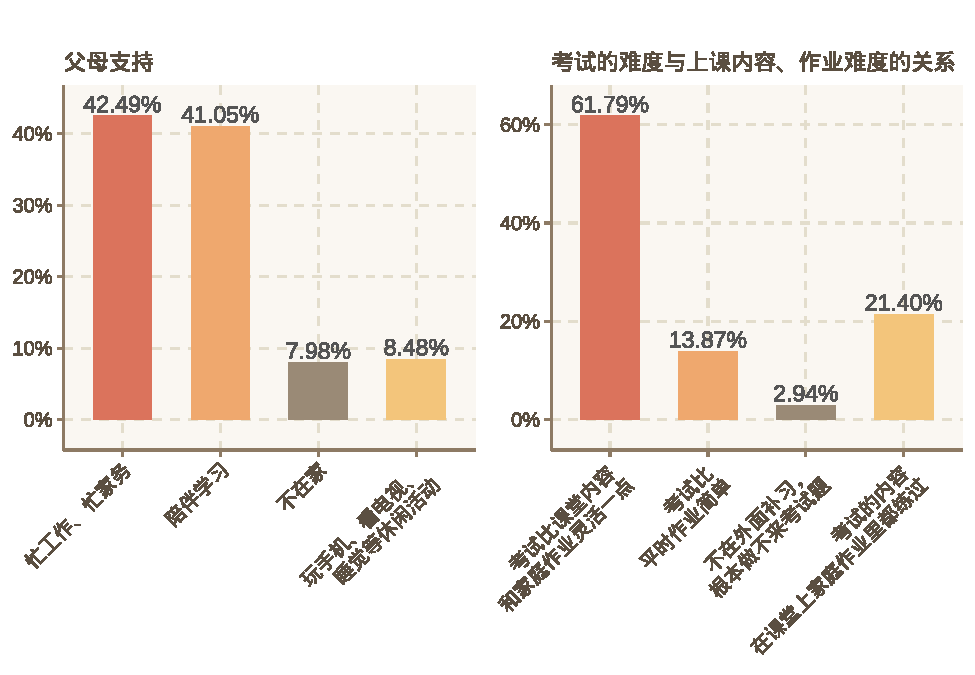
\includegraphics[width=0.99\linewidth]{ElegantBookdown_files/figure-latex/unnamed-chunk-27-1} \end{center}

\hypertarget{section-9}{%
\section{课业负担、学习方法与学业成绩的关联分析}\label{section-9}}

\hypertarget{section-10}{%
\subsection{客观学习负担与学业成绩}\label{section-10}}

根据睡眠时间、体育锻炼时间与成绩的数据叠加趋势,大部分成绩较好的学生集中于睡眠时间和体育锻炼时间较多的对应区间。

\begin{center}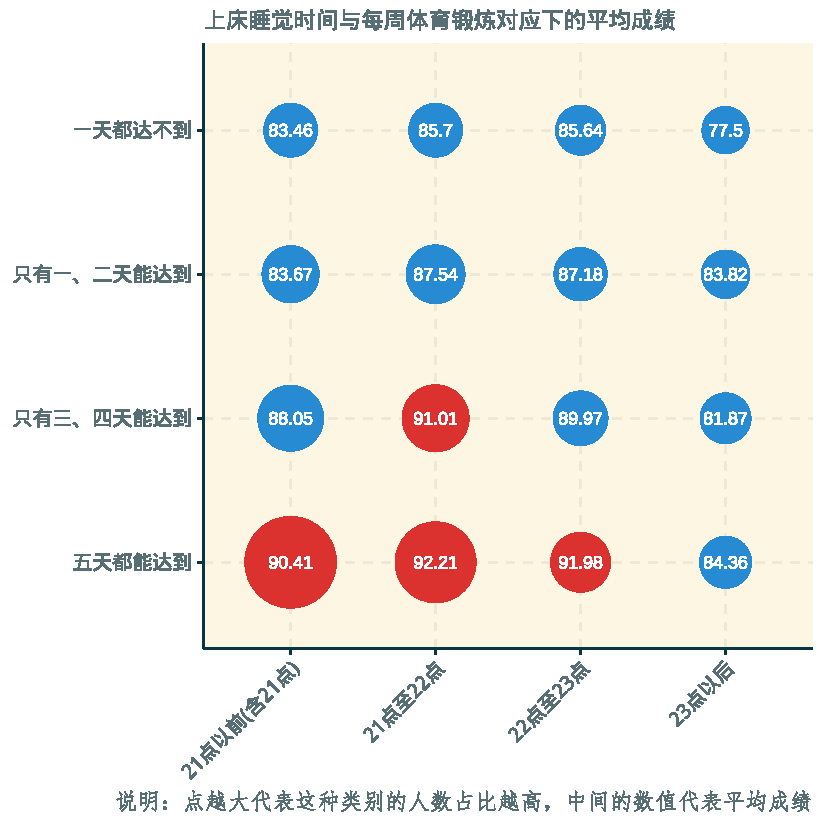
\includegraphics[width=0.99\linewidth]{ElegantBookdown_files/figure-latex/unnamed-chunk-28-1} \end{center}

根据客观负担指标达标率和学业成绩的分类统计结果,7所学校负担相对较低成绩相对较好,9所学校负担相对较低但成绩相对较低,8所学校负担相对较高成绩相对较好,10所学校负担相对较高成绩相对较低。具体学校分类如下:

\begin{center}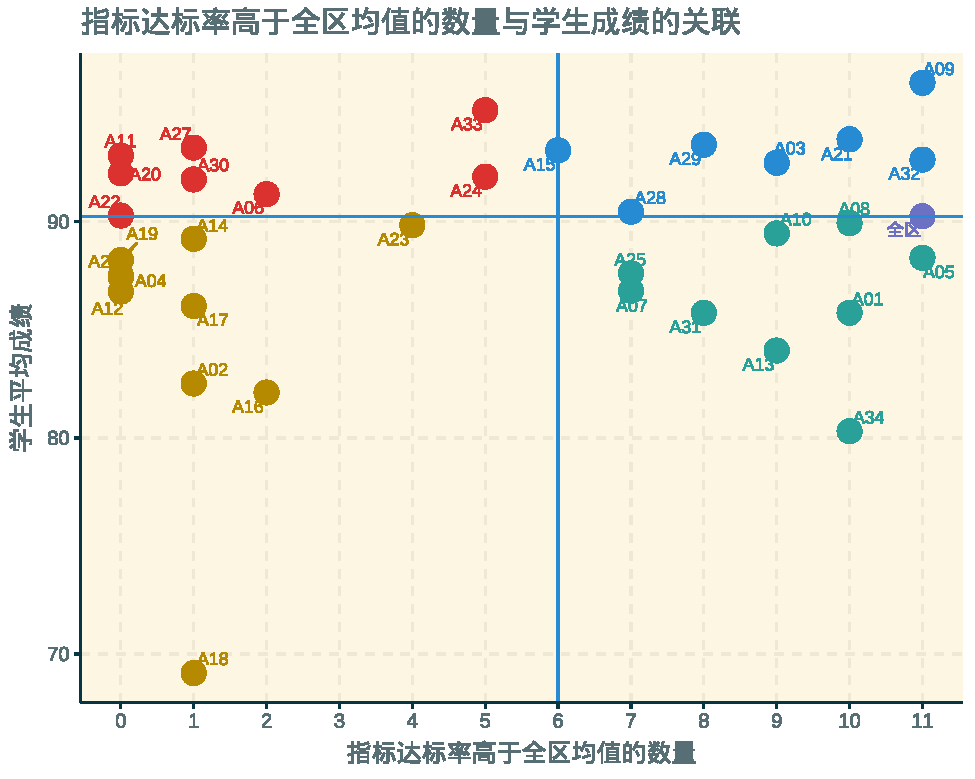
\includegraphics[width=0.99\linewidth]{ElegantBookdown_files/figure-latex/unnamed-chunk-30-1} \end{center}

以学生课后所有学习时间为自变量,以学生学业成绩为因变量进行回归分析,模型不显著(P = 0.103 \textgreater{} 0.05),表明课后学习时间与学业成绩的线性关系不明显,并非课后学习时间越长成绩越好。

\begin{center}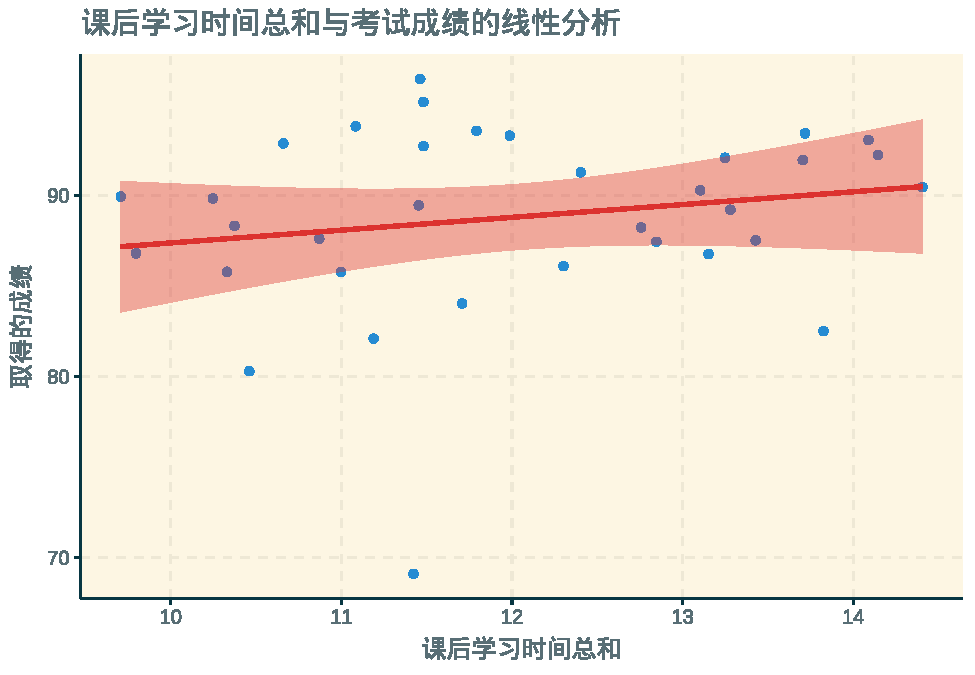
\includegraphics[width=0.99\linewidth]{ElegantBookdown_files/figure-latex/unnamed-chunk-32-1} \end{center}

\hypertarget{section-11}{%
\subsection{主观学习感受与学业成绩}\label{section-11}}

根据压力大小、负担来源与成绩的数据叠加趋势,大部分成绩较好的学生集中于没有或有一些来自自己、同学或家长的压力的对应区间。

\begin{center}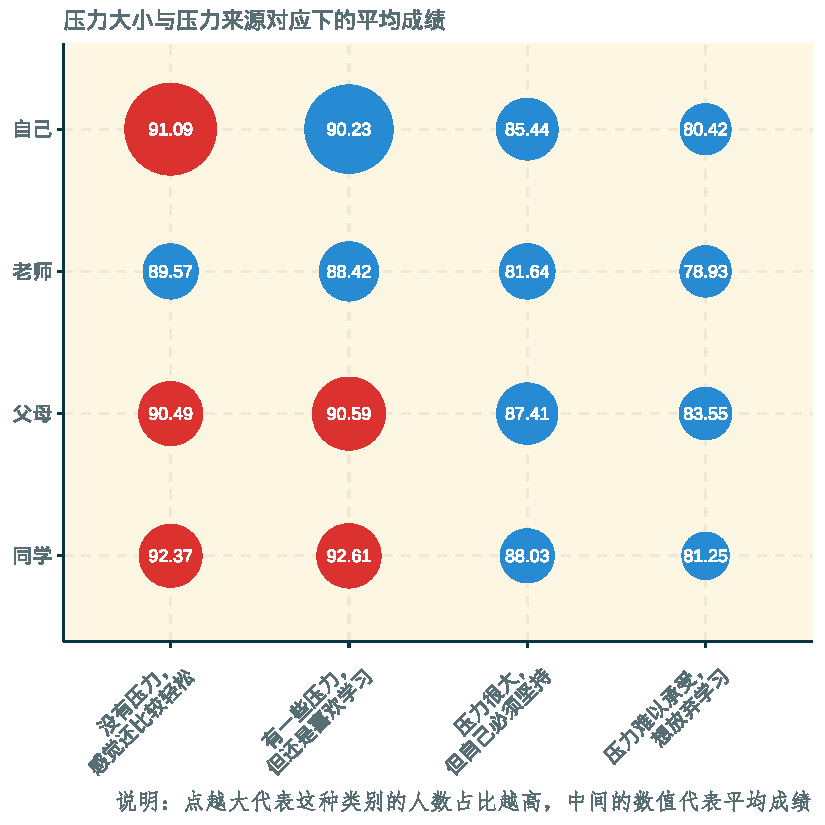
\includegraphics[width=0.99\linewidth]{ElegantBookdown_files/figure-latex/unnamed-chunk-36-1} \end{center}

根据压力大小、负担原因与成绩的数据叠加趋势,大部分成绩较好的学生集中于``没有或有一些压力''与``没有负担,或学校和课外学习相加才有负担''的对应区间。

\begin{center}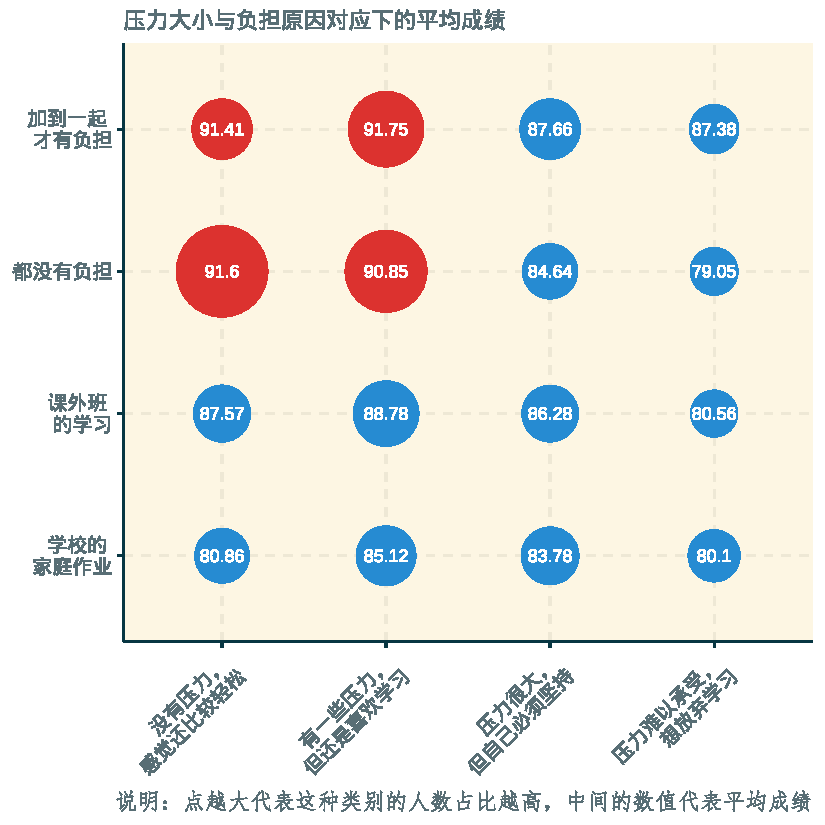
\includegraphics[width=0.99\linewidth]{ElegantBookdown_files/figure-latex/unnamed-chunk-37-1} \end{center}

\hypertarget{section-12}{%
\subsection{客观学习负担、学习深度与学业成绩}\label{section-12}}

各校对应客观学习负担达标率高于区平均的指标个数、学习深度得分率与成绩分布如下,从整
体趋势看,成绩高于区平均分的学校主要分布在学习深度得分率较高的区域,客观负担大小均
有。

\begin{center}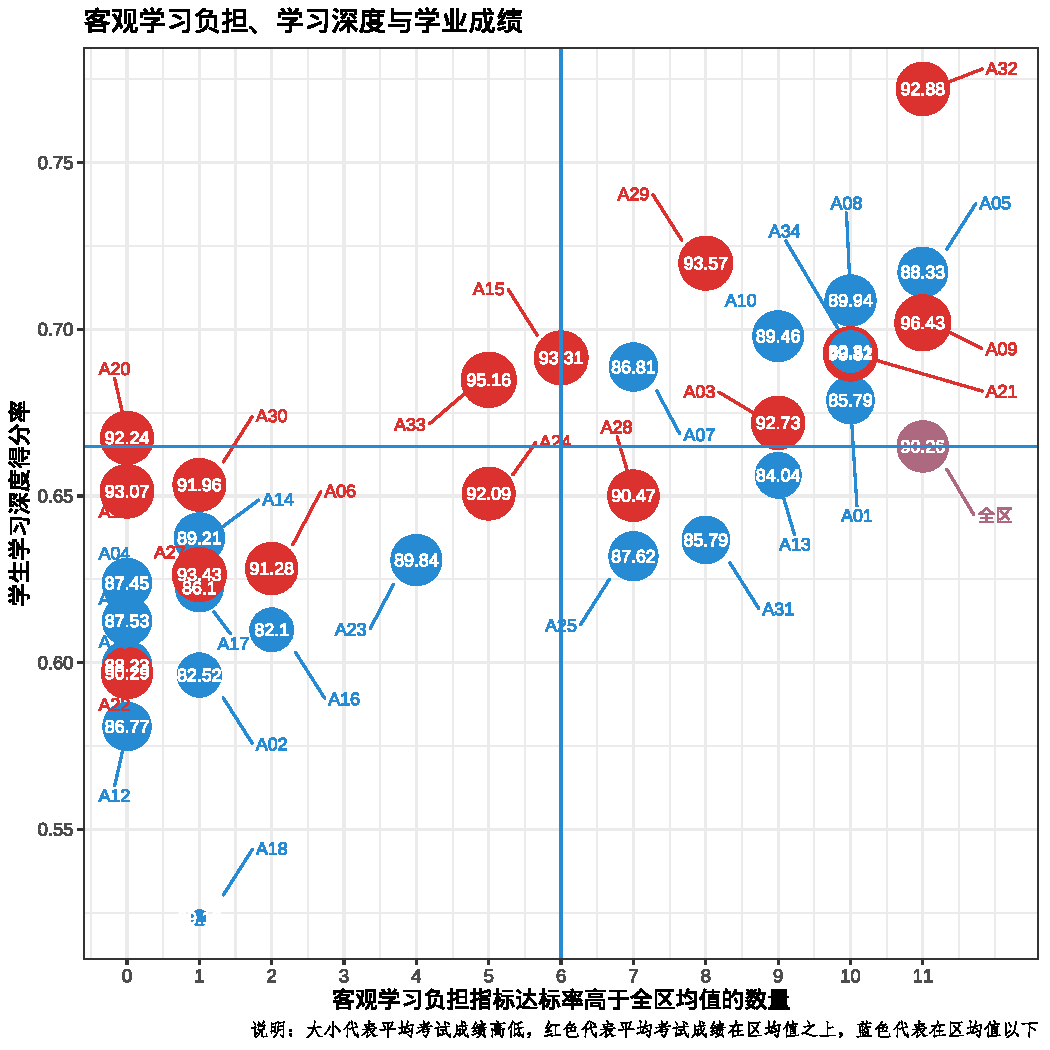
\includegraphics[width=0.99\linewidth]{ElegantBookdown_files/figure-latex/unnamed-chunk-39-1} \end{center}

\hypertarget{section-13}{%
\section{与去年的比较}\label{section-13}}

与去年相比,全区11个指标有9个指标的达标率都提高了,表明全区学生客观课业负担减少,各校在
各个客观负担指标上的得分率变化如下:

\begin{center}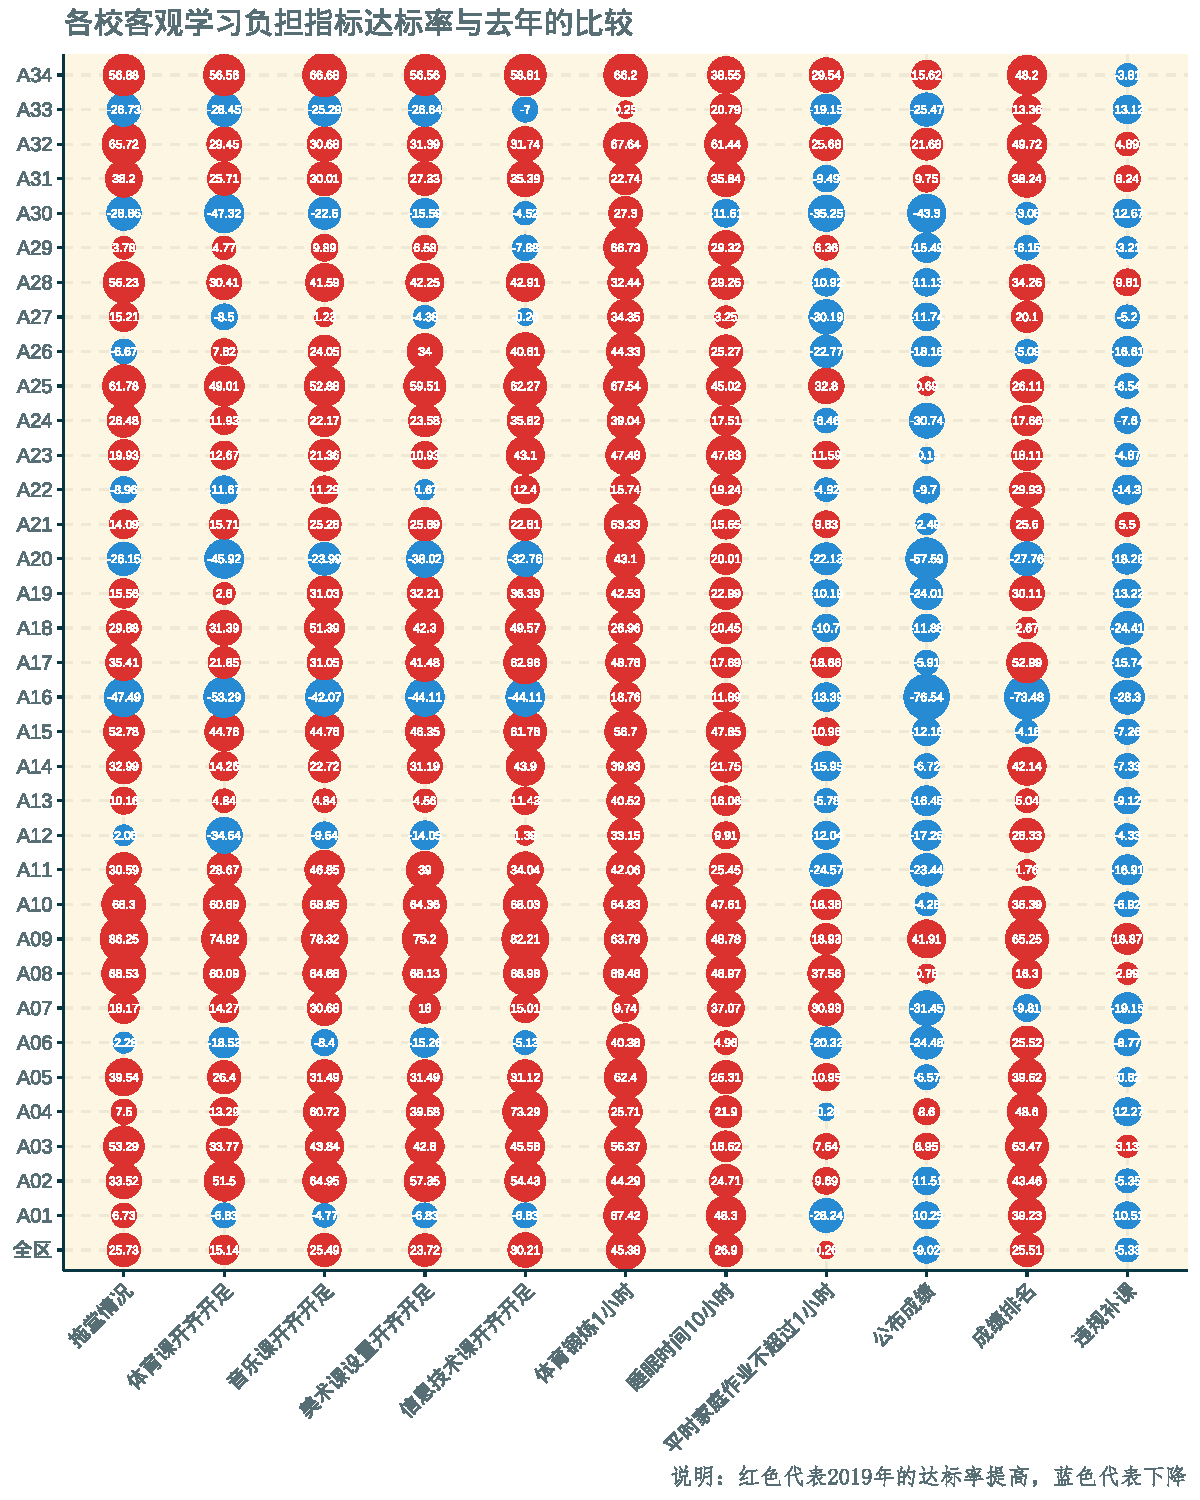
\includegraphics[width=0.99\linewidth]{ElegantBookdown_files/figure-latex/unnamed-chunk-43-1} \end{center}

\hypertarget{section-14}{%
\chapter{五年级课业负担状况}\label{section-14}}

\hypertarget{section-15}{%
\section{主要结论}\label{section-15}}

\begin{enumerate}
\def\labelenumi{\arabic{enumi}.}
\item
  在区域层面,全区五年级在 ``违规补课''、``信息技术课程开设开足'' 两个方面达标率均在 80\%
  以上,但公布成绩的达标率不足 30\%, 睡眠时间、平时作业时间的达标率低于50\%。在学校层面,
  全区34所学校中,泡桐树小学、西南财经大学附属小学、万春小学、四川师范大学实验外国语学校、鼓楼小学5所学校所有指标的达标率都高于全区平均达标率;同辉(国际)学校、实验小学青华分校、青羊实验中学附属小学、花园(国际)小学、草堂小学5所学校只有一个或两个指标低于全区平均达标率;彩虹小学、东坡小学、金沙小学3所学校所有指标的达标率都低于全区平均达标率。
\item
  五年级学生的整体存在一定学习压力,课后学习时间略高于可以承受的时间。
\item
  五年级学生学习深度的得分率为 65.65\%,学生学习的深度仍需提高。37.18\%
  的家长会在家陪伴孩子学习。
\item
  数据整体趋势表明,五年级成绩相对较好的学生主要集中在睡眠时间和体育炼
  时间较长、压力感受较低和学习深度得分率较高的区域,以客观学习负担轻为主。
\item
  与去年相比,全区 11 个客观负担指标中 8 个指标的达标率提高,3个指标降低,
  学生客观学习负担整体上降低。
\end{enumerate}

\hypertarget{section-16}{%
\section{客观学习负担情况}\label{section-16}}

\hypertarget{section-17}{%
\subsection{指标达标率情况}\label{section-17}}

在区域层面,全区五年级在``违规补课''、``信息技术课程开设开足''两个方面达标率均在80\%以上,说明较好地遵循了国家或地方有关政策规定的标准和规范。但``不公布成绩''的达标率不足30\%,``睡眠时间''和``平时作业时间''达标率低于50\%,对相关政策规定贯彻落实力度还需要大大增强。

\begin{center}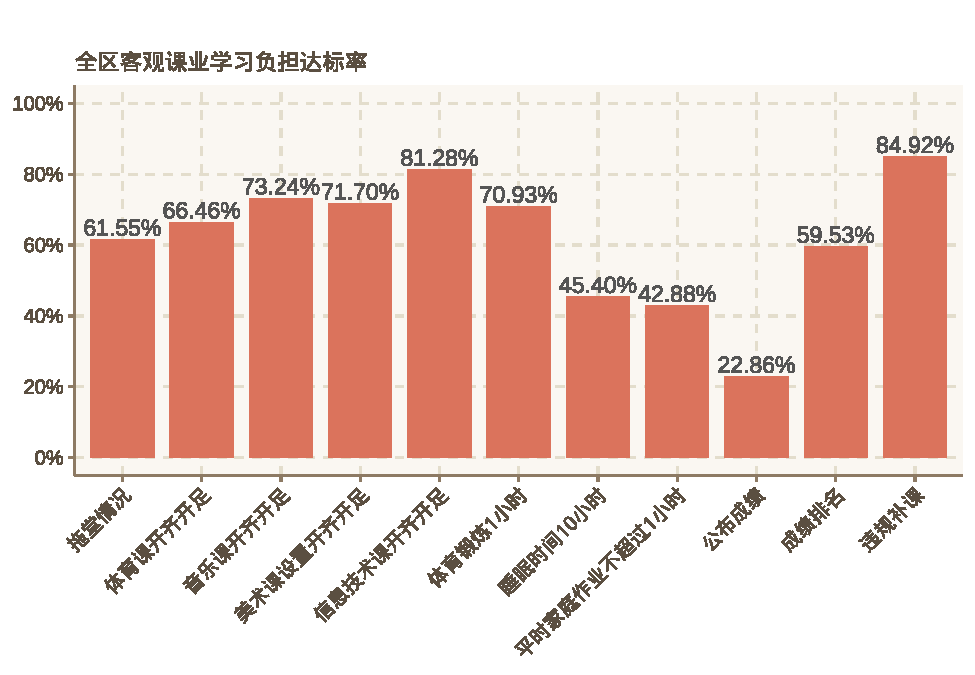
\includegraphics[width=0.99\linewidth]{ElegantBookdown_files/figure-latex/unnamed-chunk-50-1} \end{center}

根据调查结果,语文、数学、英语、其他学科的拖堂比率分别为19.36\%、27.91\%、6.78\%、5.35\%。

\begin{center}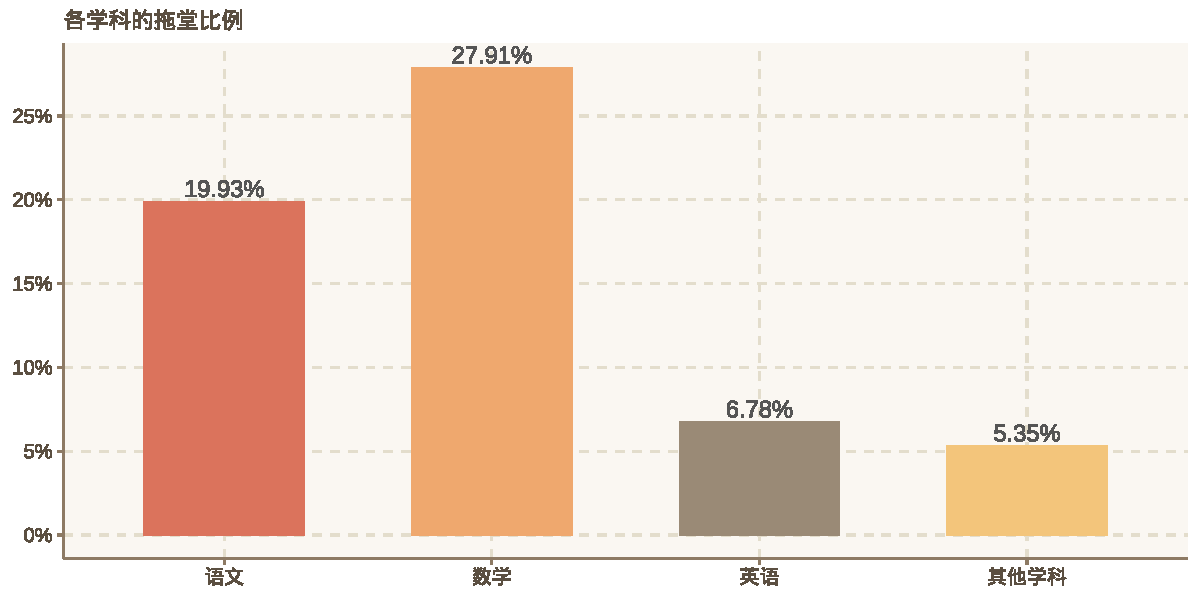
\includegraphics[width=0.99\linewidth]{ElegantBookdown_files/figure-latex/unnamed-chunk-51-1} \end{center}

根据调查结果,仍然存在少量根据考试成绩给学生排座次的情况。

\begin{center}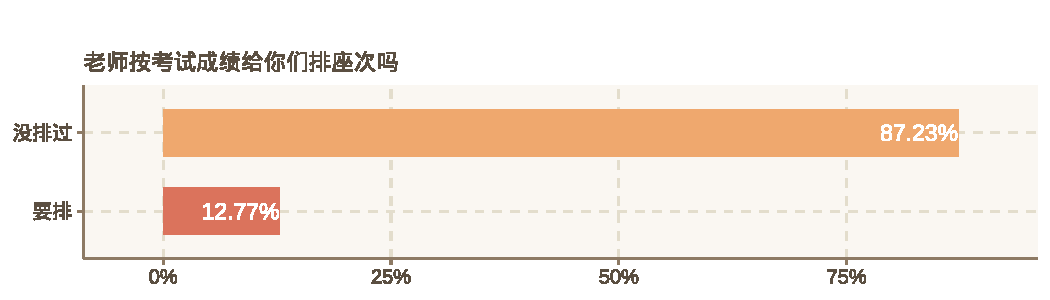
\includegraphics[width=0.99\linewidth]{ElegantBookdown_files/figure-latex/unnamed-chunk-52-1} \end{center}

针对客观学习负担 11 个指标,全区34所学校中,泡桐树小学、西南财经大学附属小学、万春小学、四川师范大学实验外国语学校、鼓楼小学5所学校所有指标的达标率都高于全区平均达标率;同辉(国际)学校、实验小学青华分校、青羊实验中学附属小学、花园(国际)小学、草堂小学5所学校只有一个或两个指标低于全区平均达标率;彩虹小学、东坡小学、金沙小学3所学校所有指标的达标率都低于全区平均达标率。

\begin{center}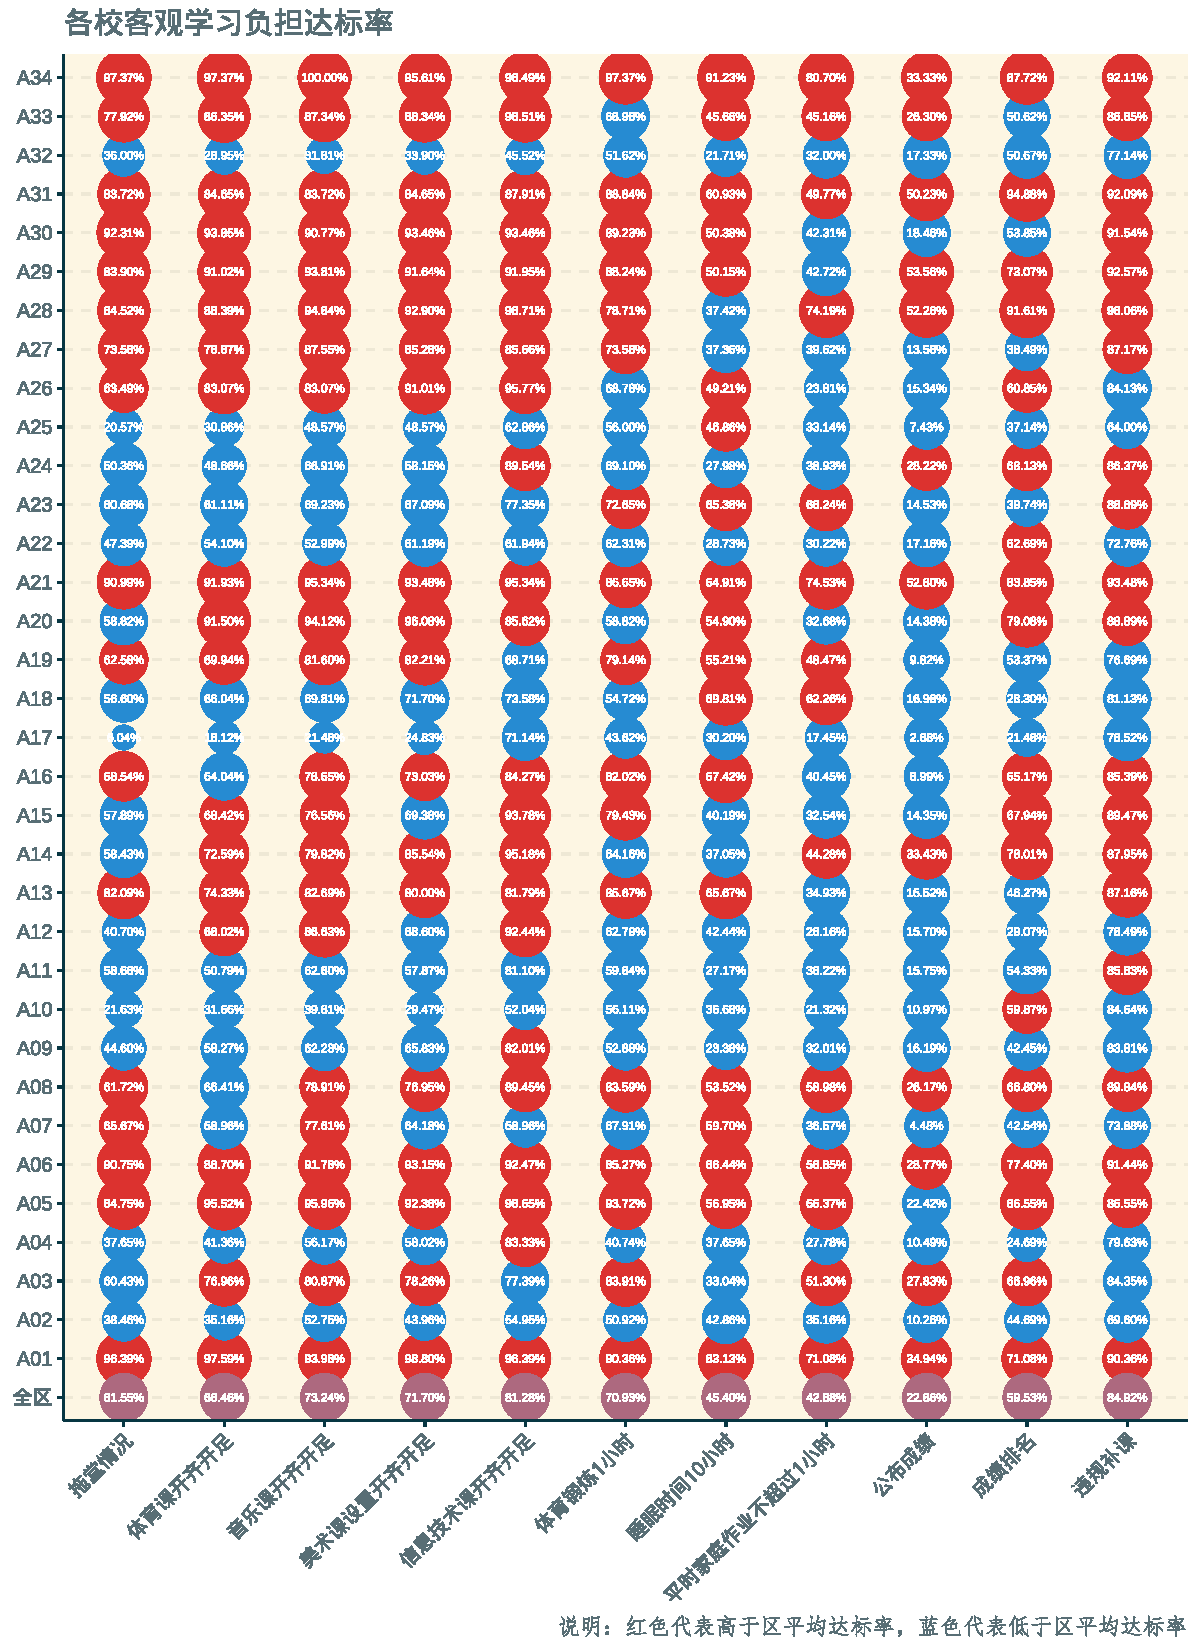
\includegraphics[width=0.99\linewidth]{ElegantBookdown_files/figure-latex/unnamed-chunk-54-1} \end{center}

\hypertarget{section-18}{%
\subsection{课外学习情况}\label{section-18}}

约80\%的五年级学生参加了至少一门文化补课,约60\%的学生一周平均文化补课时间在0-3小时之间,约70\%的学生每天文化补课作业时间在1小时内,参加文化补课的主要原因是扩展知识、拓展能力。

\begin{center}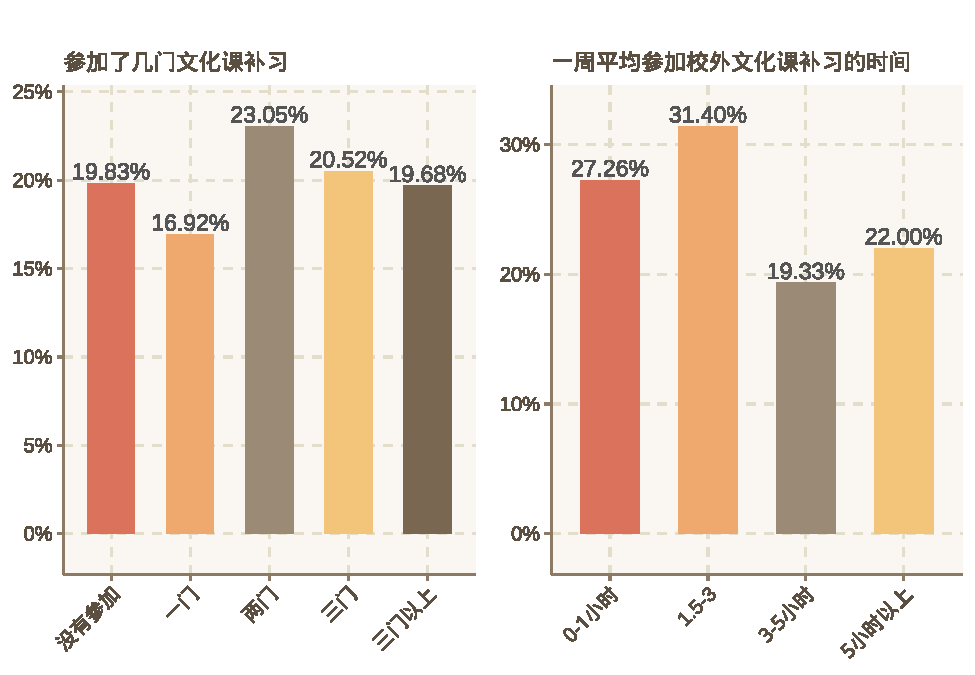
\includegraphics[width=0.99\linewidth]{ElegantBookdown_files/figure-latex/unnamed-chunk-55-1} \end{center}

\begin{center}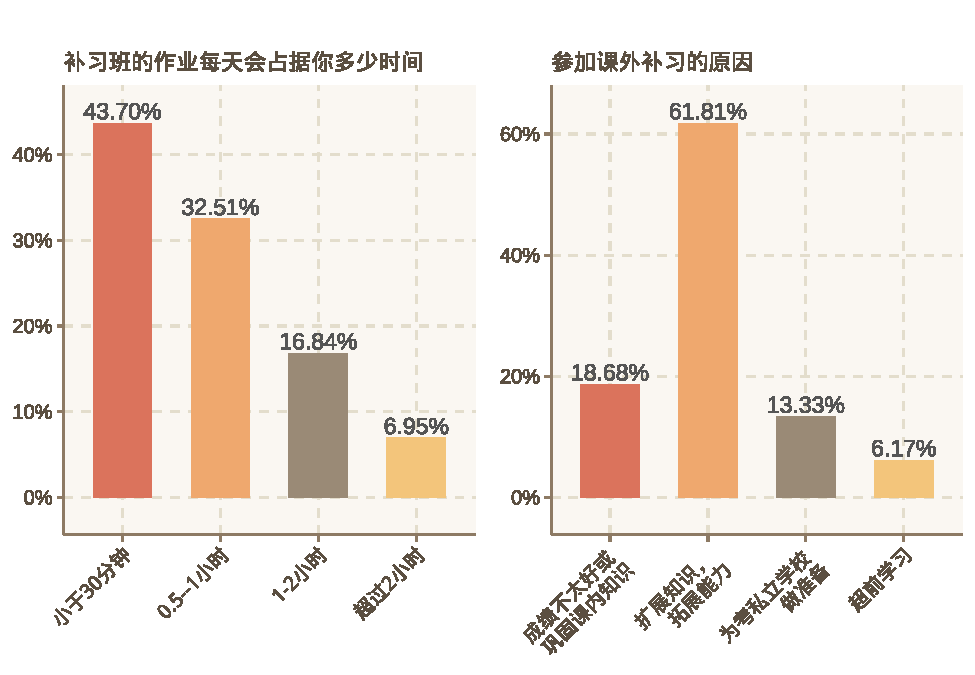
\includegraphics[width=0.99\linewidth]{ElegantBookdown_files/figure-latex/unnamed-chunk-56-1} \end{center}

五年级79.15\% 的学生参加了至少一项艺体培训,65.21\% 的学生一周平均艺体培训时间在2 小时以内。

\begin{center}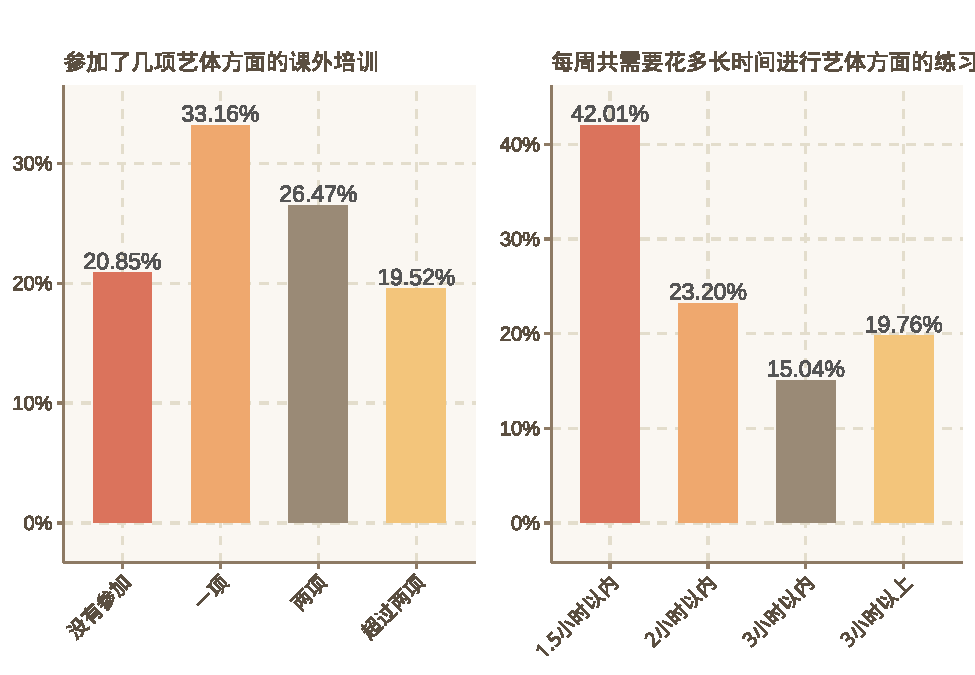
\includegraphics[width=0.99\linewidth]{ElegantBookdown_files/figure-latex/unnamed-chunk-57-1} \end{center}

\hypertarget{section-19}{%
\section{主观学习感受}\label{section-19}}

五年级学生存在一定压力,34.36\%的学生认为没有压力,53.45\%的学生有一些压力但仍喜欢学习,主要的学习压力来自自己,28.21\% 的学生认为学校和课外学习加在一起才有负担。

\begin{center}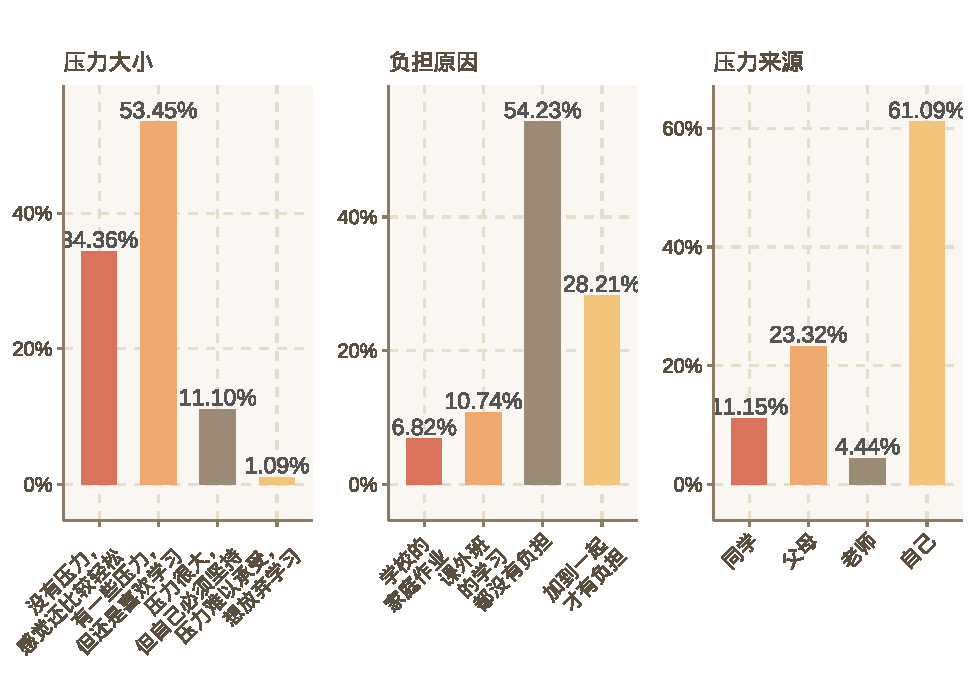
\includegraphics[width=0.99\linewidth]{ElegantBookdown_files/figure-latex/unnamed-chunk-58-1} \end{center}

各校学生学习感知的压力大小分类统计如下:

\begin{center}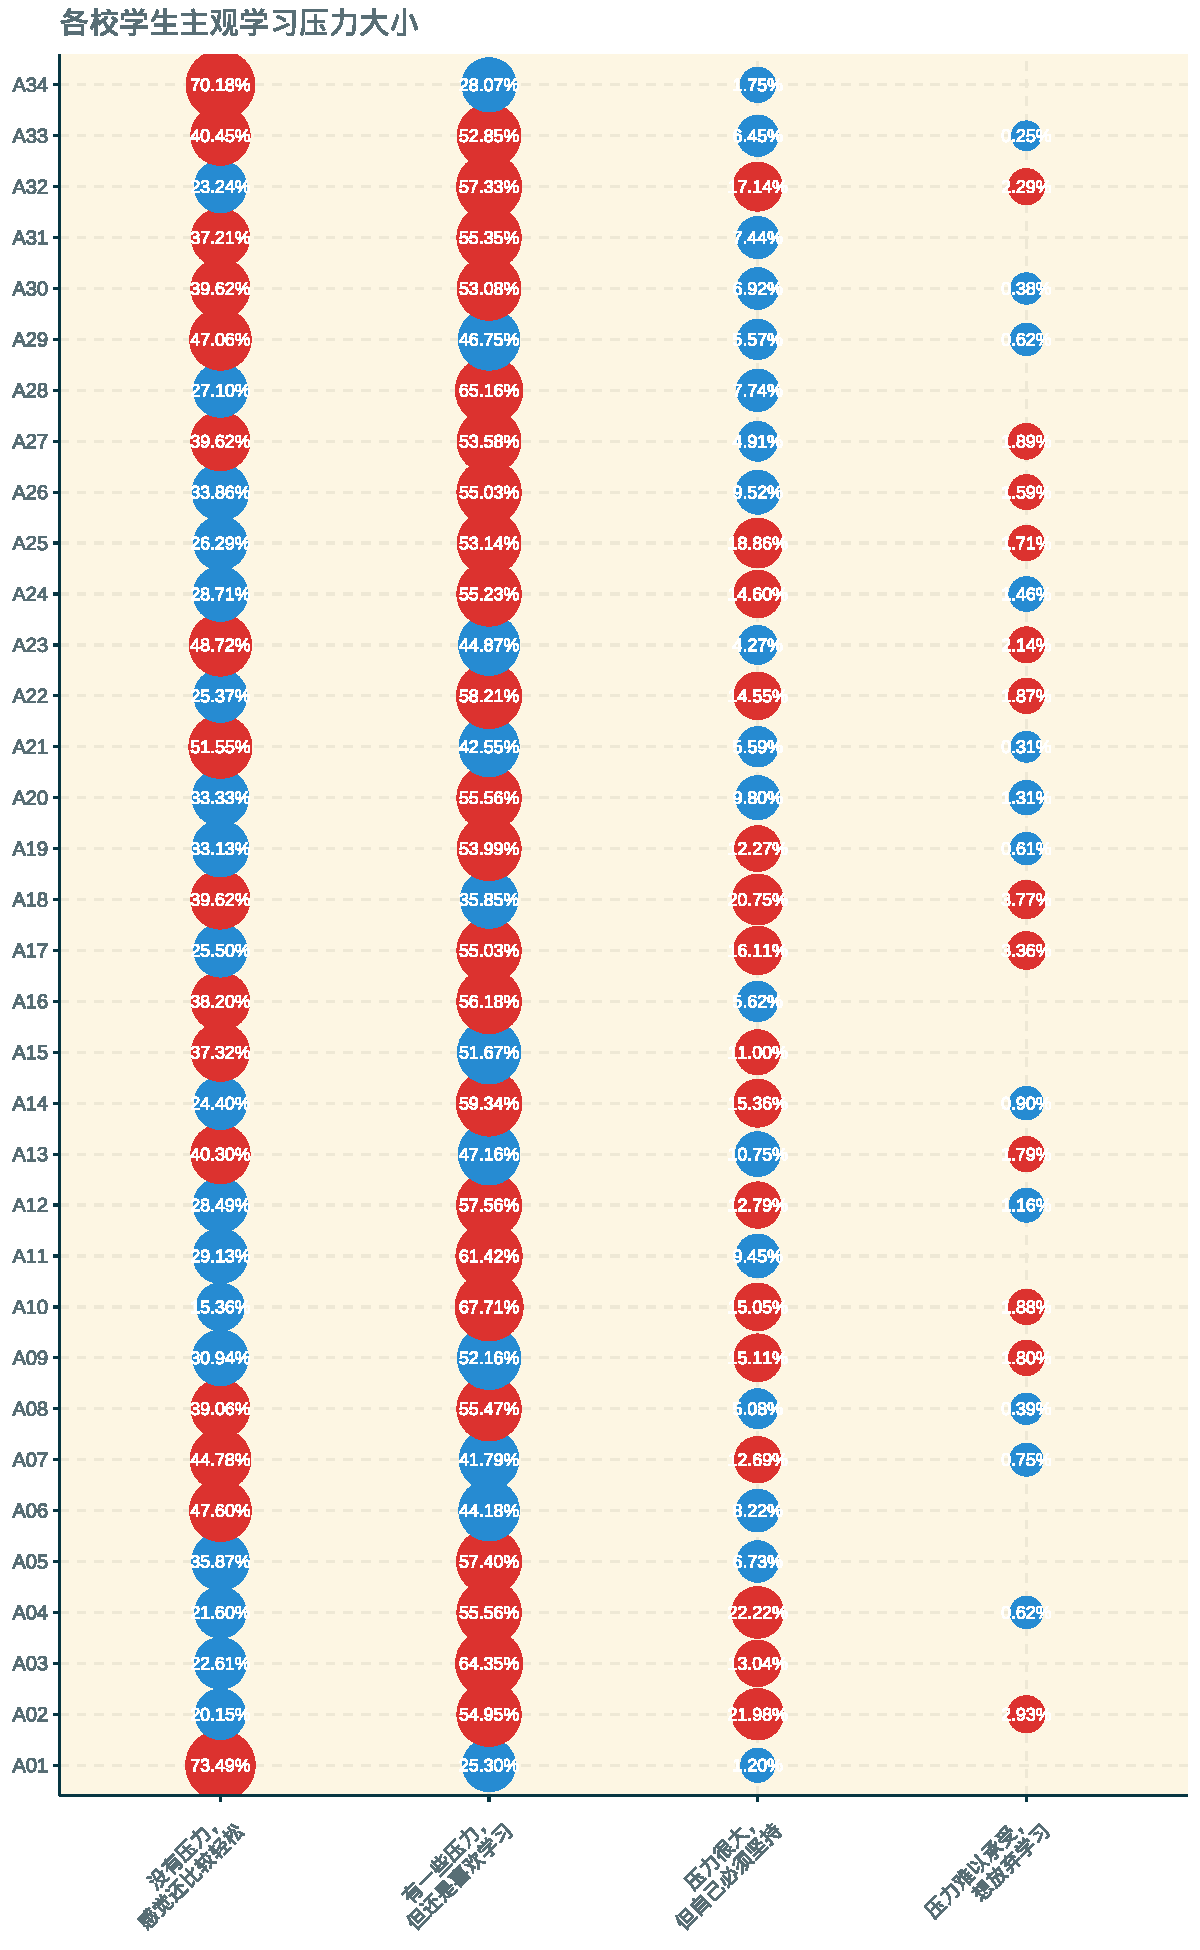
\includegraphics[width=0.99\linewidth]{ElegantBookdown_files/figure-latex/unnamed-chunk-62-1} \end{center}

大部分五年级学生对文化补课和艺体培训接受度和兴趣比较高。

\begin{center}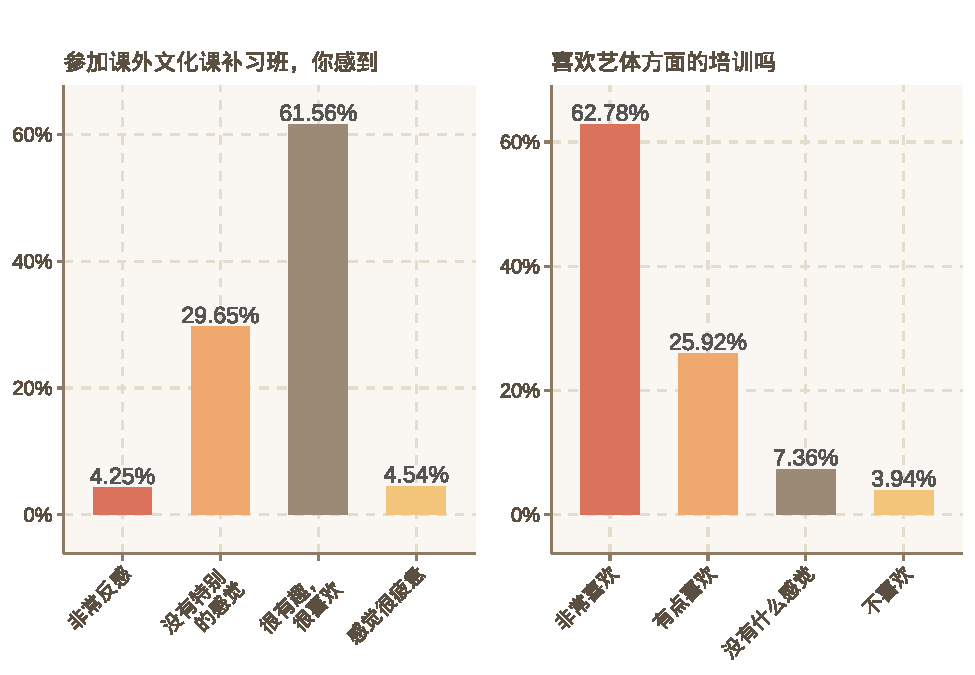
\includegraphics[width=0.99\linewidth]{ElegantBookdown_files/figure-latex/unnamed-chunk-63-1} \end{center}

将完成所有学校作业、补习班课程、补习班作业、艺体方面的练习的时间加和,与学生可以接受的负担时间进行比较,从全区来看,学生心理预期承受时间为平均每周12.41小时,实际支出实际12.7小时,两者相差不大,表明平均而言放学后的学业负荷学生基本能承受。

各校学生实际课后学习时间和能承受的时间及其差值统计如下:

\begin{table}[!h]

\caption{\label{tab:unnamed-chunk-66}各校课外补习实际支出时间与心理预期统计}
\centering
\fontsize{12}{14}\selectfont
\begin{tabular}{lccc}
\toprule
学校 & \makecell[c]{每周实际 \\ 补习时间} & \makecell[c]{每周可承受 \\ 补习时间} & \makecell[c]{超过可承受 \\ 时间}\\
\midrule
\rowcolor{gray!6}  A01 & 8.84 & 10.21 & \multicolumn{1}{r}{\cellcolor[HTML]{F3C57B}{\textcolor{black}{-1.37}}}\\
A02 & 12.78 & 12.28 & \multicolumn{1}{r}{\cellcolor[HTML]{db735c}{\textcolor{black}{0.5}}}\\
\rowcolor{gray!6}  A03 & 12.27 & 12.78 & \multicolumn{1}{r}{\cellcolor[HTML]{F3C57B}{\textcolor{black}{-0.51}}}\\
A04 & 14.22 & 12.64 & \multicolumn{1}{r}{\cellcolor[HTML]{db735c}{\textcolor{black}{1.58}}}\\
\rowcolor{gray!6}  A05 & 11.00 & 12.36 & \multicolumn{1}{r}{\cellcolor[HTML]{F3C57B}{\textcolor{black}{-1.36}}}\\
A06 & 11.58 & 12.39 & \multicolumn{1}{r}{\cellcolor[HTML]{F3C57B}{\textcolor{black}{-0.81}}}\\
\rowcolor{gray!6}  A07 & 12.38 & 11.34 & \multicolumn{1}{r}{\cellcolor[HTML]{db735c}{\textcolor{black}{1.04}}}\\
A08 & 11.24 & 12.73 & \multicolumn{1}{r}{\cellcolor[HTML]{F3C57B}{\textcolor{black}{-1.49}}}\\
\rowcolor{gray!6}  A09 & 14.83 & 12.81 & \multicolumn{1}{r}{\cellcolor[HTML]{db735c}{\textcolor{black}{2.02}}}\\
A10 & 13.79 & 11.86 & \multicolumn{1}{r}{\cellcolor[HTML]{db735c}{\textcolor{black}{1.93}}}\\
\rowcolor{gray!6}  A11 & 13.49 & 12.61 & \multicolumn{1}{r}{\cellcolor[HTML]{db735c}{\textcolor{black}{0.89}}}\\
A12 & 13.55 & 12.54 & \multicolumn{1}{r}{\cellcolor[HTML]{db735c}{\textcolor{black}{1.01}}}\\
\rowcolor{gray!6}  A13 & 13.17 & 13.00 & \multicolumn{1}{r}{\cellcolor[HTML]{db735c}{\textcolor{black}{0.16}}}\\
A14 & 12.80 & 12.27 & \multicolumn{1}{r}{\cellcolor[HTML]{db735c}{\textcolor{black}{0.53}}}\\
\rowcolor{gray!6}  A15 & 13.58 & 12.98 & \multicolumn{1}{r}{\cellcolor[HTML]{db735c}{\textcolor{black}{0.6}}}\\
A16 & 11.48 & 11.15 & \multicolumn{1}{r}{\cellcolor[HTML]{db735c}{\textcolor{black}{0.33}}}\\
\rowcolor{gray!6}  A17 & 14.51 & 11.07 & \multicolumn{1}{r}{\cellcolor[HTML]{db735c}{\textcolor{black}{3.45}}}\\
A18 & 8.58 & 9.67 & \multicolumn{1}{r}{\cellcolor[HTML]{F3C57B}{\textcolor{black}{-1.09}}}\\
\rowcolor{gray!6}  A19 & 12.27 & 11.90 & \multicolumn{1}{r}{\cellcolor[HTML]{db735c}{\textcolor{black}{0.37}}}\\
A20 & 12.11 & 12.03 & \multicolumn{1}{r}{\cellcolor[HTML]{db735c}{\textcolor{black}{0.08}}}\\
\rowcolor{gray!6}  A21 & 9.93 & 12.40 & \multicolumn{1}{r}{\cellcolor[HTML]{F3C57B}{\textcolor{black}{-2.47}}}\\
A22 & 13.76 & 11.47 & \multicolumn{1}{r}{\cellcolor[HTML]{db735c}{\textcolor{black}{2.29}}}\\
\rowcolor{gray!6}  A23 & 9.50 & 10.88 & \multicolumn{1}{r}{\cellcolor[HTML]{F3C57B}{\textcolor{black}{-1.38}}}\\
A24 & 14.49 & 13.80 & \multicolumn{1}{r}{\cellcolor[HTML]{db735c}{\textcolor{black}{0.68}}}\\
\rowcolor{gray!6}  A25 & 13.11 & 11.75 & \multicolumn{1}{r}{\cellcolor[HTML]{db735c}{\textcolor{black}{1.36}}}\\
A26 & 12.68 & 11.57 & \multicolumn{1}{r}{\cellcolor[HTML]{db735c}{\textcolor{black}{1.11}}}\\
\rowcolor{gray!6}  A27 & 13.07 & 13.18 & \multicolumn{1}{r}{\cellcolor[HTML]{F3C57B}{\textcolor{black}{-0.11}}}\\
A28 & 12.27 & 12.52 & \multicolumn{1}{r}{\cellcolor[HTML]{F3C57B}{\textcolor{black}{-0.25}}}\\
\rowcolor{gray!6}  A29 & 13.14 & 13.86 & \multicolumn{1}{r}{\cellcolor[HTML]{F3C57B}{\textcolor{black}{-0.72}}}\\
A30 & 12.62 & 13.21 & \multicolumn{1}{r}{\cellcolor[HTML]{F3C57B}{\textcolor{black}{-0.59}}}\\
\rowcolor{gray!6}  A31 & 11.56 & 12.17 & \multicolumn{1}{r}{\cellcolor[HTML]{F3C57B}{\textcolor{black}{-0.62}}}\\
A32 & 15.03 & 12.81 & \multicolumn{1}{r}{\cellcolor[HTML]{db735c}{\textcolor{black}{2.22}}}\\
\rowcolor{gray!6}  A33 & 12.06 & 11.65 & \multicolumn{1}{r}{\cellcolor[HTML]{db735c}{\textcolor{black}{0.41}}}\\
A34 & 8.80 & 13.25 & \multicolumn{1}{r}{\cellcolor[HTML]{F3C57B}{\textcolor{black}{-4.44}}}\\
\bottomrule
\multicolumn{4}{l}{\textsuperscript{a} 单位:小时}\\
\end{tabular}
\end{table}

\cleardoublepage

\hypertarget{section-20}{%
\section{学习方法}\label{section-20}}

\hypertarget{section-21}{%
\subsection{学生学习深度}\label{section-21}}

对考查学生学习深度的量表式题目进行因素分析,根据因素分析得到的因子载荷合成学习深度总分,计算得到学生学习深度得分率。全区五年级学生学习深度的得分率为65.65\%,整
体并不高,表明学生学习的深度不够。各校得分率最高的为 77.50\%,最低的为 54.49\%,具体得分率如下:

\begin{center}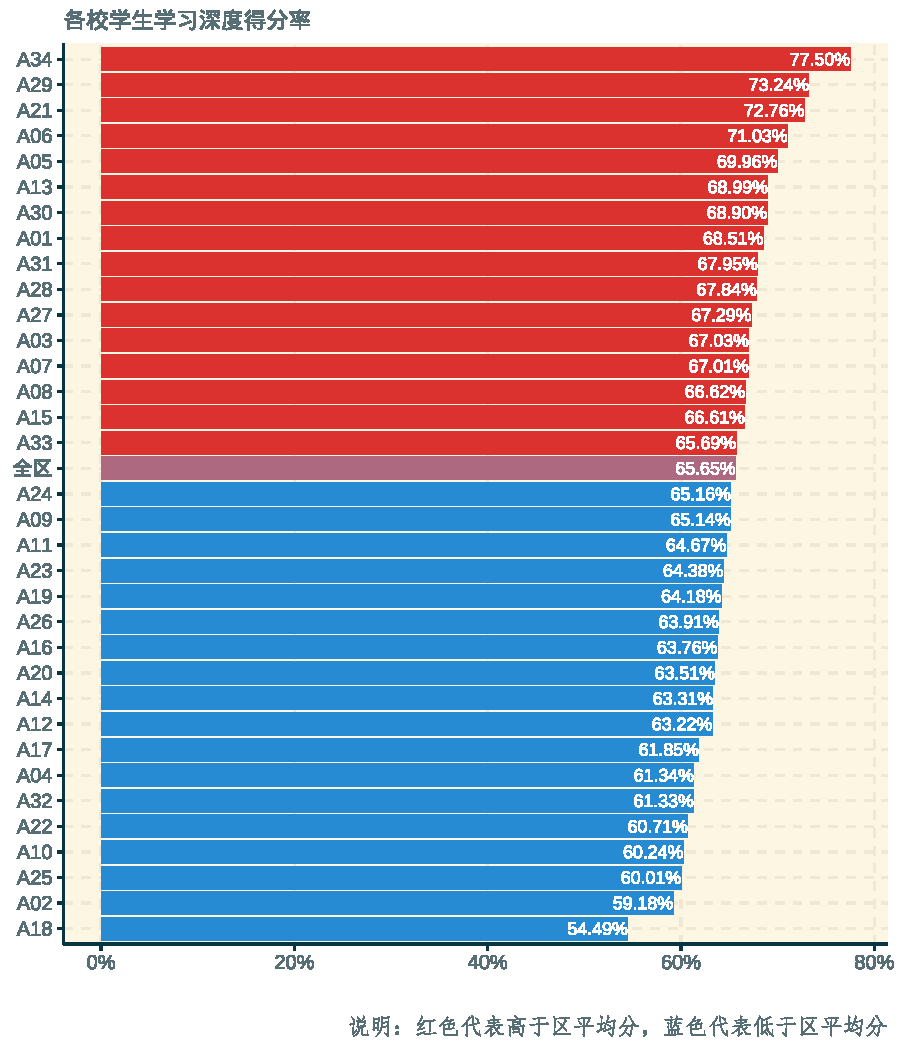
\includegraphics[width=0.99\linewidth]{ElegantBookdown_files/figure-latex/unnamed-chunk-69-1} \end{center}

\hypertarget{section-22}{%
\subsection{学生作业完成情况}\label{section-22}}

对于学生完成作业,约80\%的学生都认为自己是专心致志一鼓作气做完,在正确率方面差别不大。值得注意的是,约60\%学生认为考试比课堂内容和家庭作业灵活一些。此外,37.18\%的家长会在家陪伴孩子学习。

\begin{center}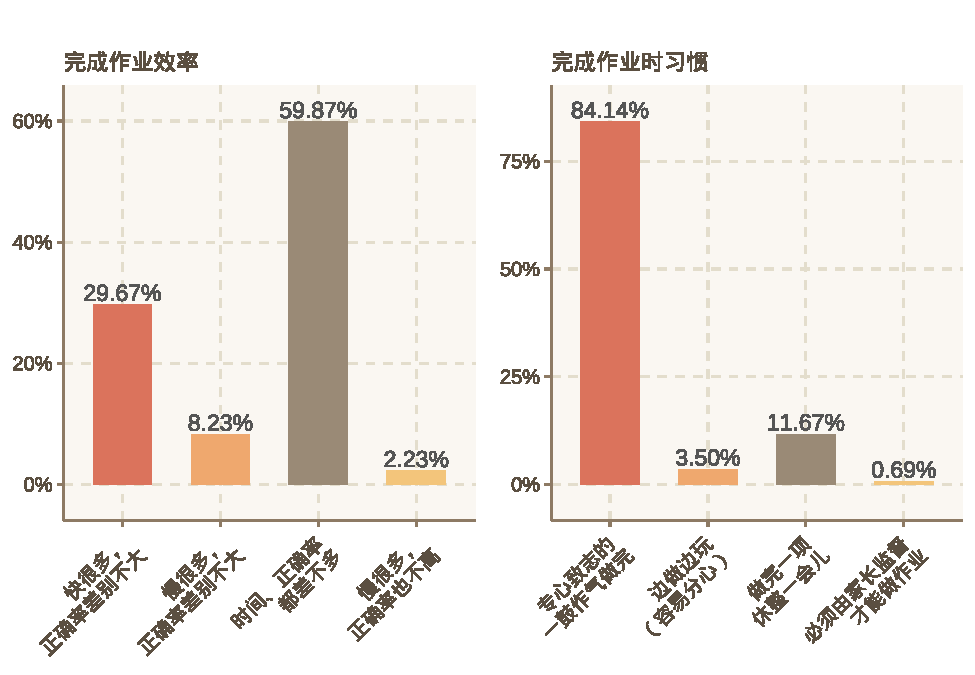
\includegraphics[width=0.99\linewidth]{ElegantBookdown_files/figure-latex/unnamed-chunk-70-1} \end{center}

\begin{center}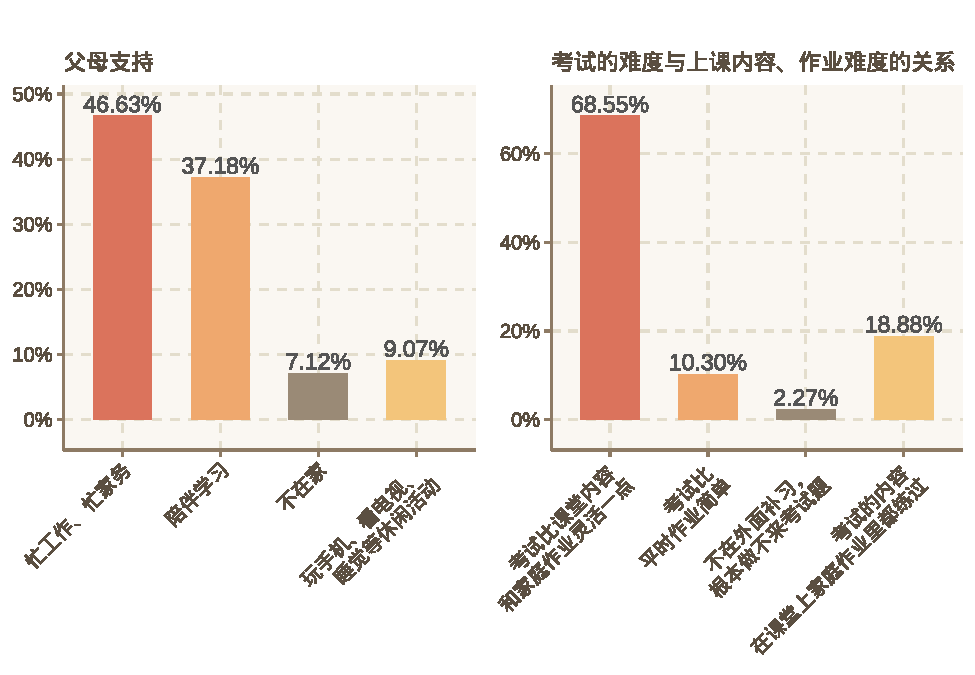
\includegraphics[width=0.99\linewidth]{ElegantBookdown_files/figure-latex/unnamed-chunk-71-1} \end{center}

\hypertarget{section-23}{%
\section{课业负担、学习方法与学业成绩的关联分析}\label{section-23}}

\hypertarget{section-24}{%
\subsection{客观学习负担与学业成绩}\label{section-24}}

根据睡眠时间、体育锻炼时间与成绩的数据叠加趋势,大部分成绩较好的学生集中于睡眠时间和体育锻炼时间较多的对应区间。

\begin{center}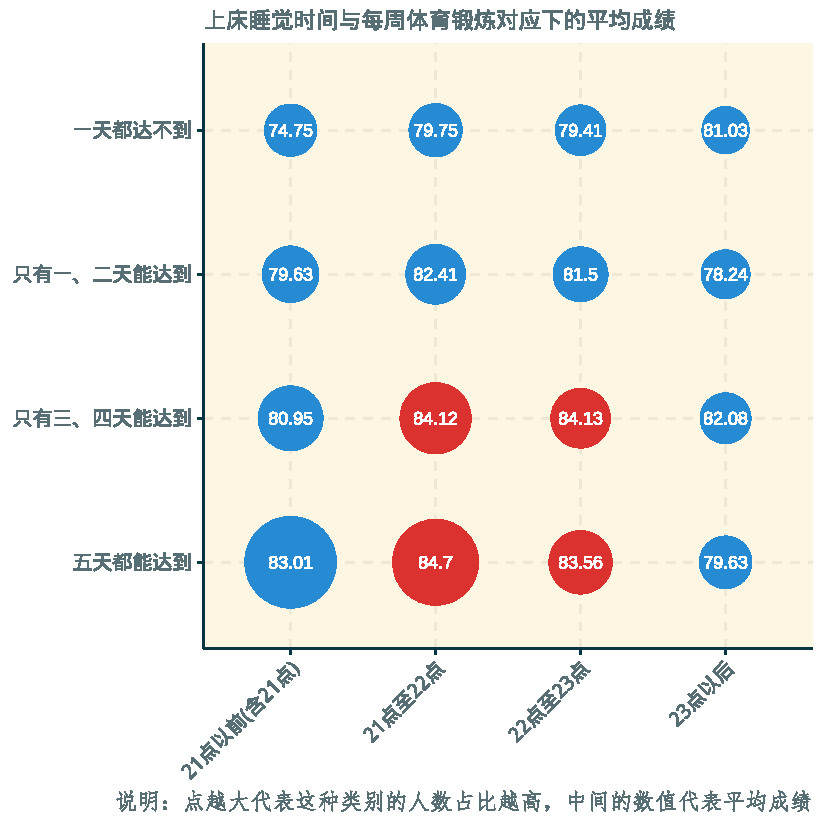
\includegraphics[width=0.99\linewidth]{ElegantBookdown_files/figure-latex/unnamed-chunk-72-1} \end{center}

根据客观负担指标达标率和学业成绩的分类统计结果,9所学校负担相对较低成绩相对较好,11所学校负担相对较低但成绩相对较低,6所学校负担相对较高成绩相对较好,8所学校负担相对较高成绩相对较低。具体学校分类如下:

\begin{center}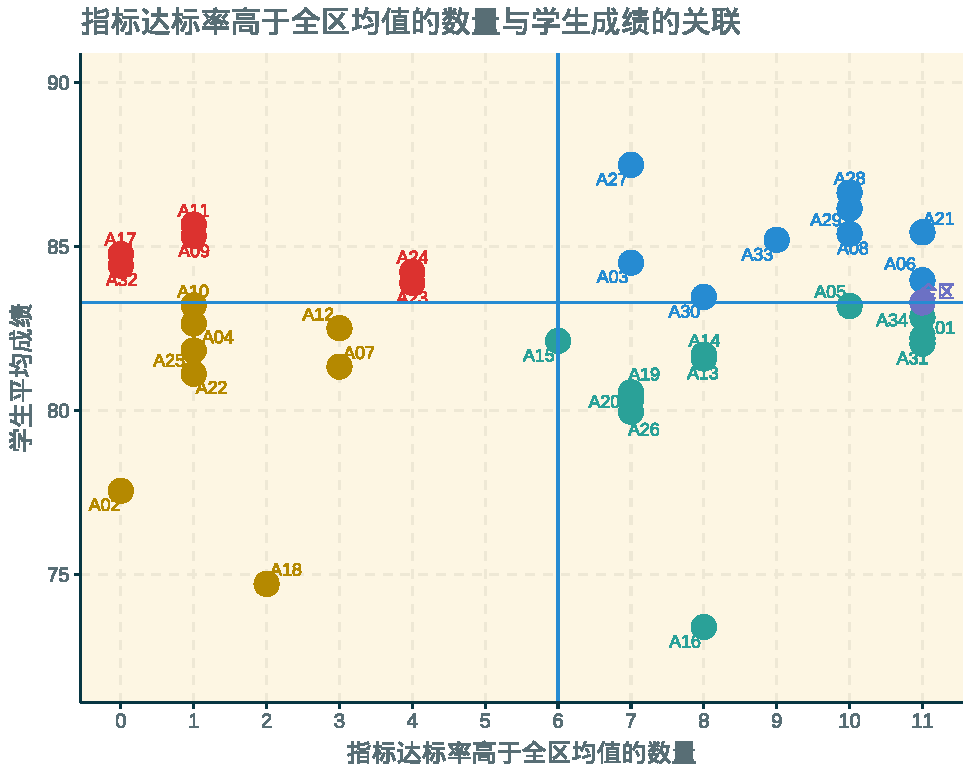
\includegraphics[width=0.99\linewidth]{ElegantBookdown_files/figure-latex/unnamed-chunk-74-1} \end{center}

以学生课后所有学习时间为自变量,以学生学业成绩为因变量进行回归分析,模型不显著(P = 0.141 \textgreater{} 0.05),表明课后学习时间与学业成绩的线性关系不明显,并非课后学习时间越长成绩越好。

\begin{center}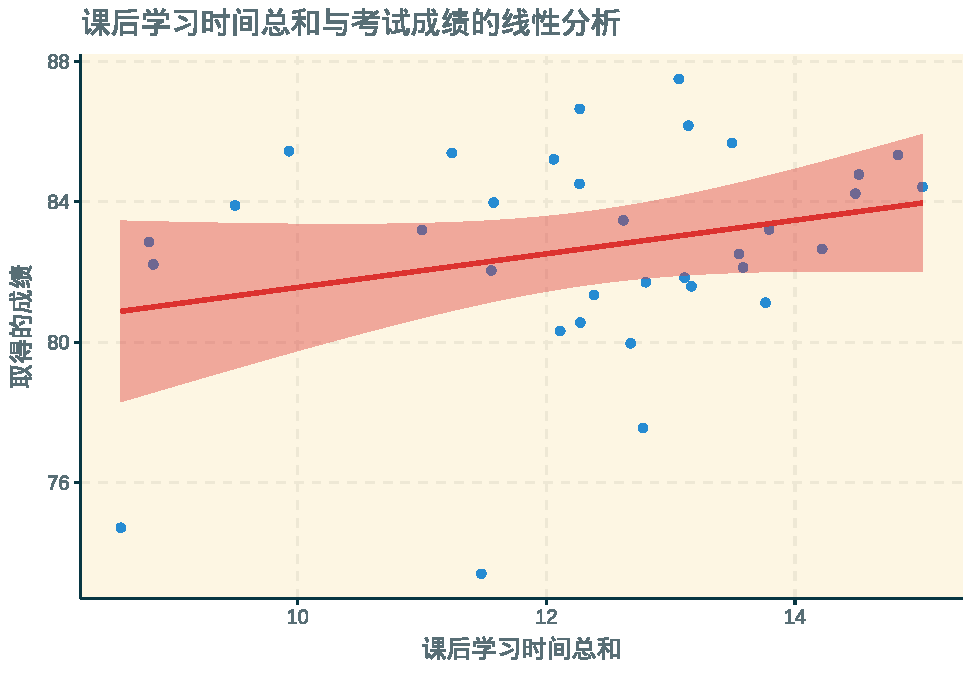
\includegraphics[width=0.99\linewidth]{ElegantBookdown_files/figure-latex/unnamed-chunk-76-1} \end{center}

\hypertarget{section-25}{%
\subsection{主观学习感受与学业成绩}\label{section-25}}

根据压力大小、负担来源与成绩的数据叠加趋势,大部分成绩较好的学生集中于没有或有一些来自自己、同学或家长的压力的对应区间。

\begin{center}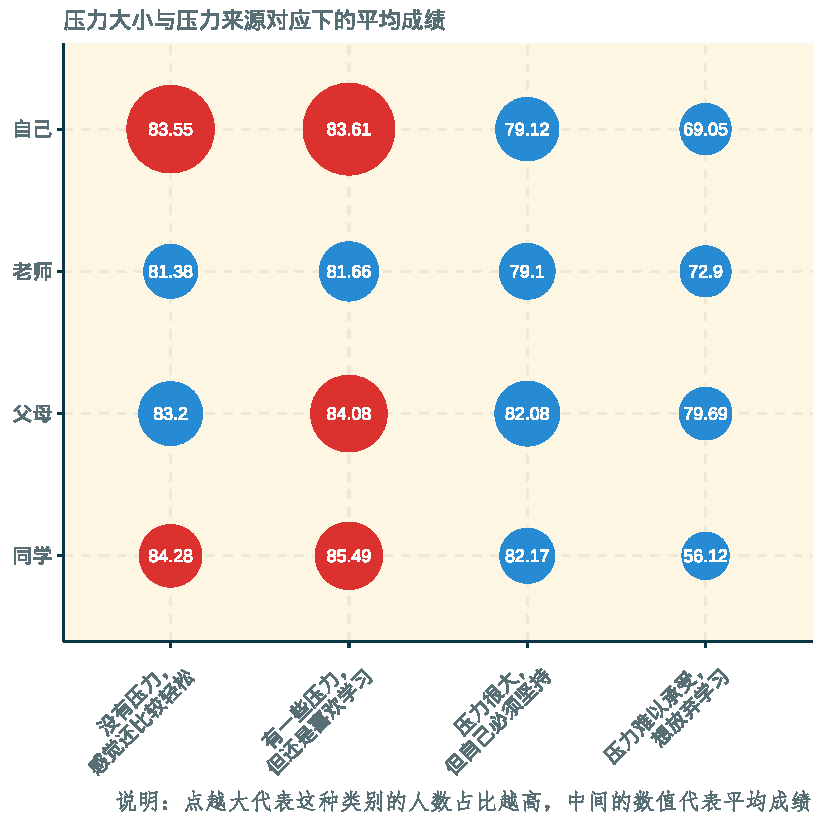
\includegraphics[width=0.99\linewidth]{ElegantBookdown_files/figure-latex/unnamed-chunk-80-1} \end{center}

根据压力大小、负担原因与成绩的数据叠加趋势,大部分成绩较好的学生集中于``没有或有一些压力'' 与 ``没有或有一些来自学校和课外学习相加才有负担''的对应区间。

\begin{center}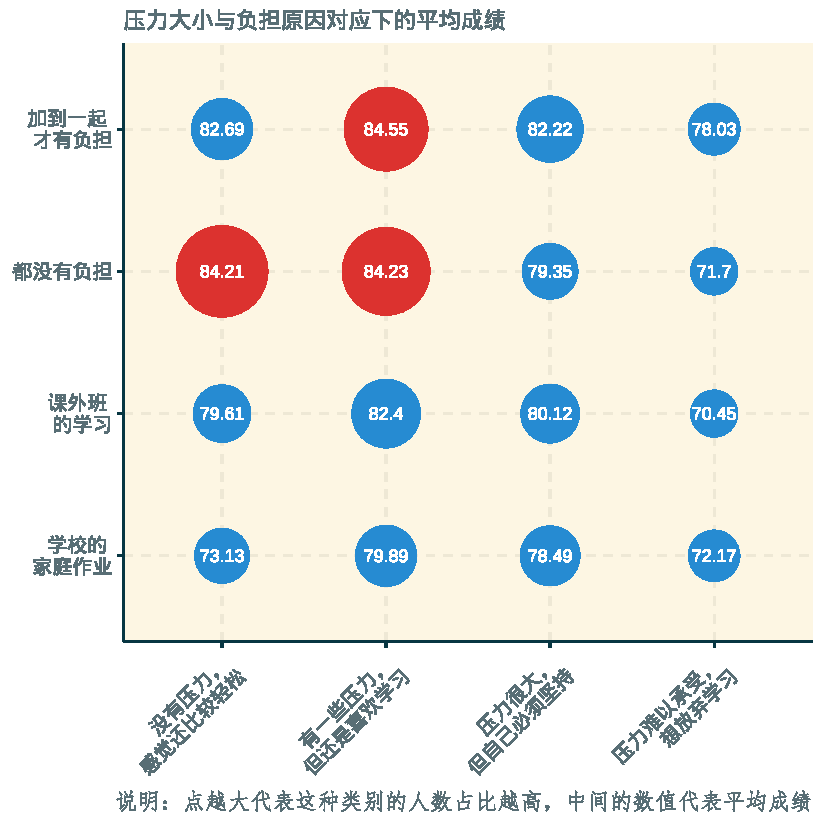
\includegraphics[width=0.99\linewidth]{ElegantBookdown_files/figure-latex/unnamed-chunk-81-1} \end{center}

\hypertarget{section-26}{%
\subsection{客观学习负担、学习深度与学业成绩}\label{section-26}}

各校对应客观学习负担达标率高于区平均的指标个数、学习深度得分率与成绩分布如下,从整
体趋势看,成绩高于区平均分的学校主要分布在学习深度得分率较高以及以客观学习负担轻为主的区域。

\begin{center}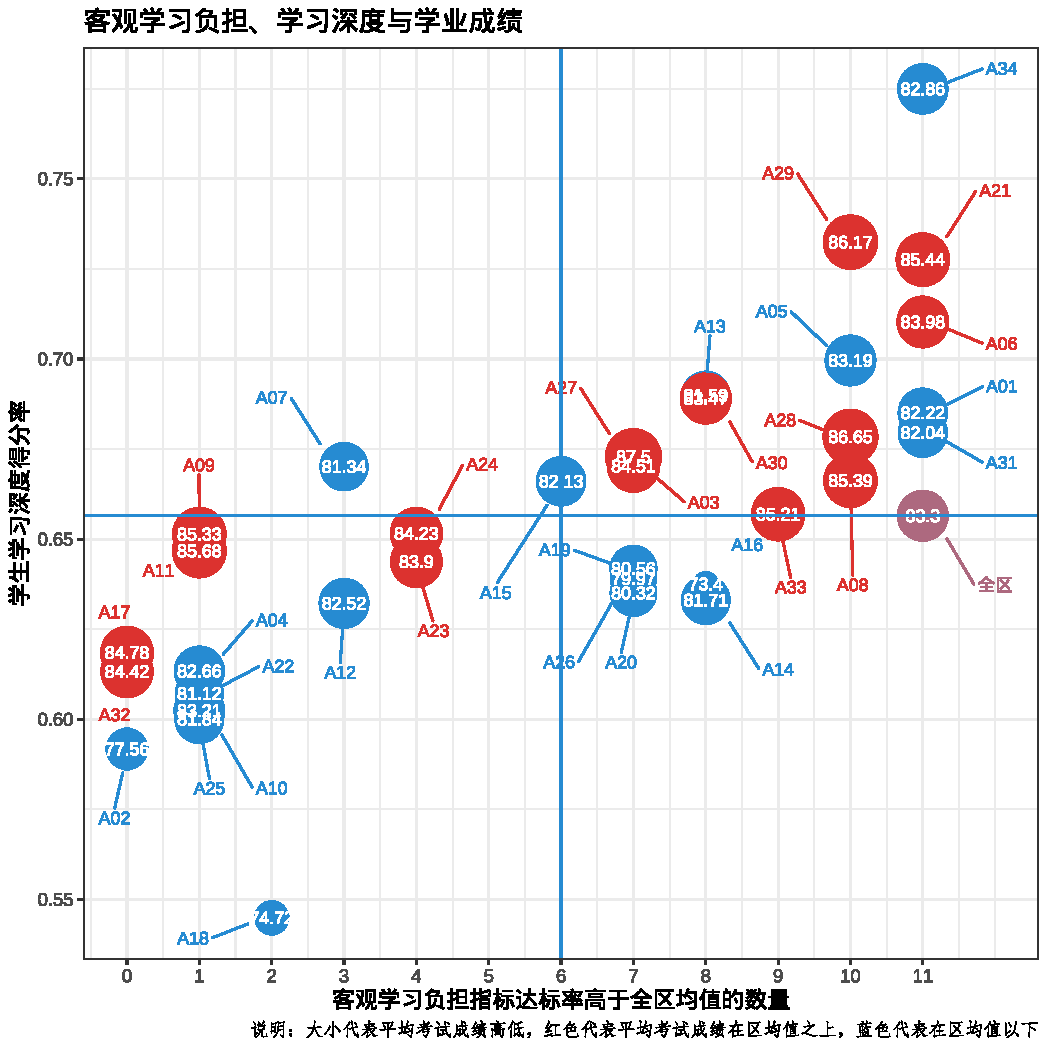
\includegraphics[width=0.99\linewidth]{ElegantBookdown_files/figure-latex/unnamed-chunk-83-1} \end{center}

\hypertarget{section-27}{%
\section{与去年的比较}\label{section-27}}

与去年相比,全区11个指标有8个指标的达标率都提高了,表明全区学生客观课业负担减少,各校在
各个客观负担指标上的得分率变化如下:

\begin{center}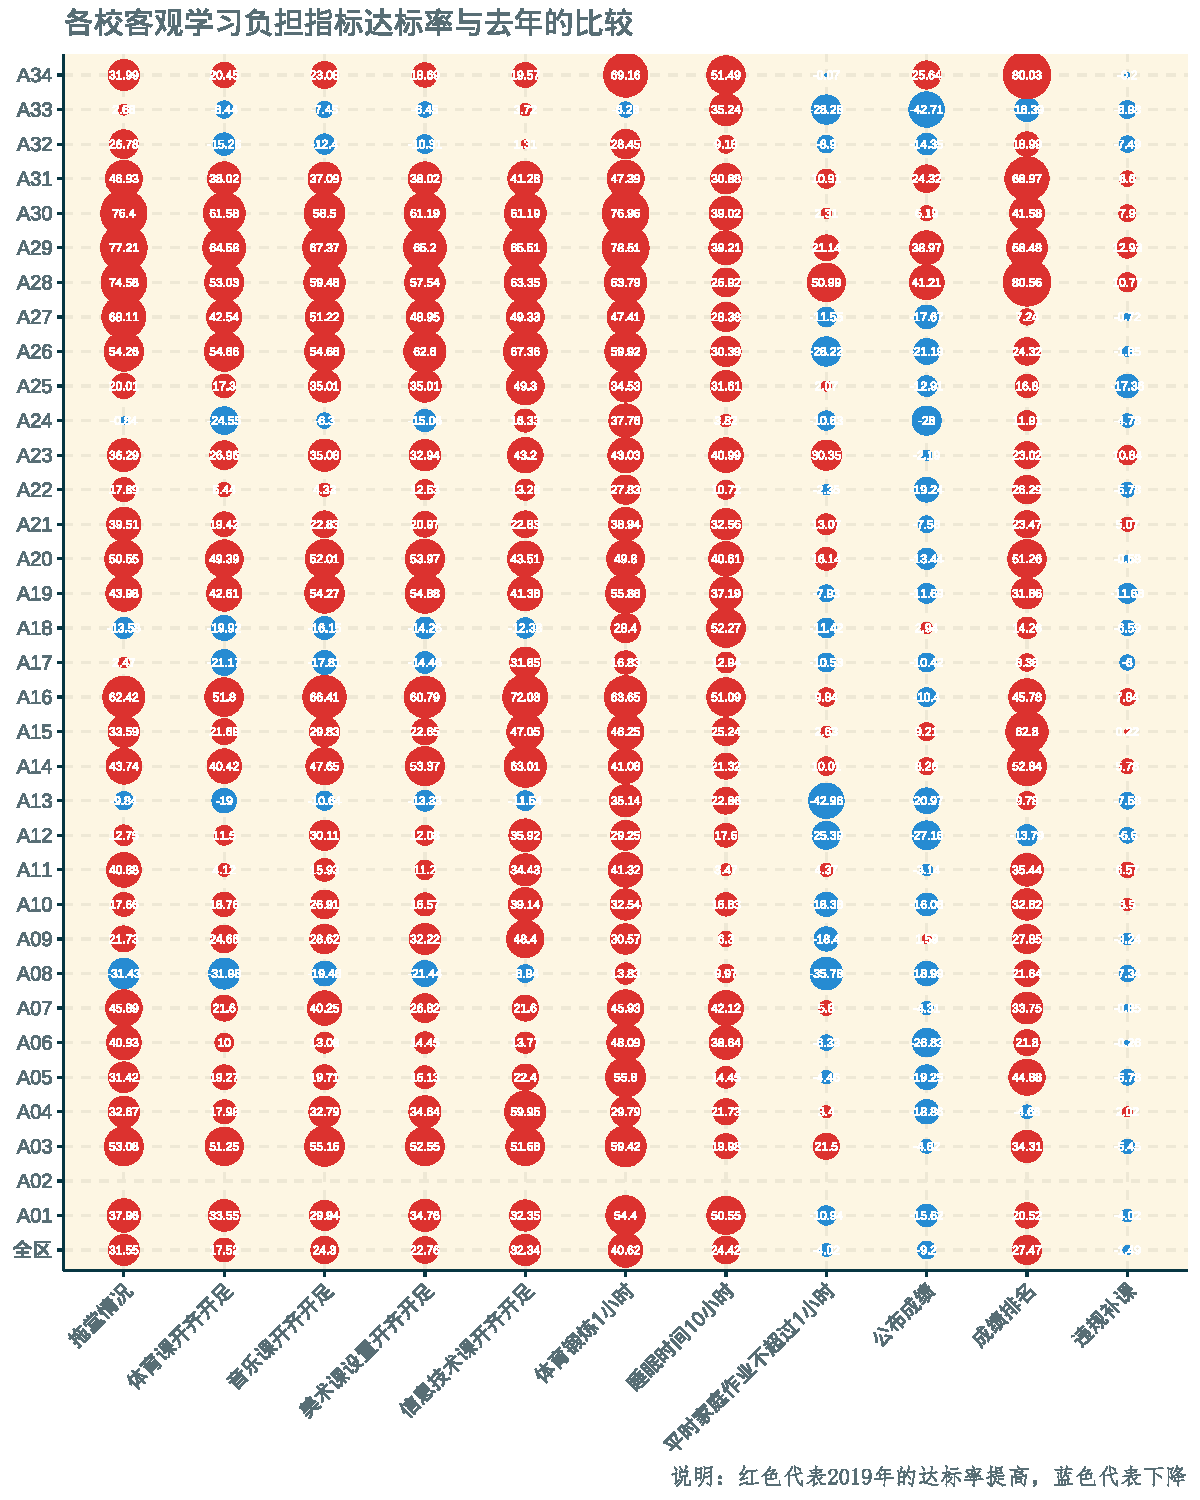
\includegraphics[width=0.99\linewidth]{ElegantBookdown_files/figure-latex/unnamed-chunk-87-1} \end{center}
% 参考文献
\bibliography{book.bib}



% 插入 after_body.tex

\end{document}
